\documentclass[amsmath, amssymb, aps, floatfix, nofootinbib, preprintnumbers,showpacs, superscriptaddress, twocolumn]{revtex4-1}
\usepackage{bm}
\usepackage[cmyk]{xcolor}
\usepackage{dcolumn}
\usepackage{epsfig}
\usepackage{float}
\usepackage{graphicx}
\usepackage{multirow}
\usepackage{subfigure}

\newcommand{\D}{\operatorname{d\!}}
\newcommand{\ket}[1]{| #1 \rangle}
\newcommand{\bra}[1]{\langle #1 |}
\newcommand{\braket}[2]{\langle #1 | #2\rangle}
\newcommand{\normord}[1]{\mathopen: #1 \mathclose:}

\begin{document}

\title{Studies of quantum dots}

\author{Fei Yuan}
\affiliation{National Superconducting Cyclotron Laboratory and
  Department of Physics and Astronomy,
  Michigan State University,
  East Lansing, MI 48824, USA}
\author{J\o rgen H\o gberget}
\affiliation{Department of Physics, University of Oslo, N-0316 Oslo, Norway}
\author{Sam Novario}
\affiliation{National Superconducting Cyclotron Laboratory and
  Department of Physics and Astronomy,
  Michigan State University,
  East Lansing, MI 48824, USA}
\author{Nathan Parzuchowski}
\affiliation{National Superconducting Cyclotron Laboratory and
  Department of Physics and Astronomy,
  Michigan State University,
  East Lansing, MI 48824, USA}
\author{Sarah Reimann}
\affiliation{Department of Chemistry and Center for Theoretical and Computational Chemistry, University of Oslo, N-0316 Oslo, Norway}
\author{Scott Bogner}
\affiliation{National Superconducting Cyclotron Laboratory and
  Department of Physics and Astronomy,
  Michigan State University,
  East Lansing, MI 48824, USA}
\author{Morten Hjorth-Jensen}
\affiliation{National Superconducting Cyclotron Laboratory and
  Department of Physics and Astronomy,
  Michigan State University,
  East Lansing, MI 48824, USA}
\affiliation{Department of Physics, University of Oslo, N-0316 Oslo, Norway}


\begin{abstract}
  We present and compare several many-body methods used to study a quantum dot
  system.  We calculate the approximate ground state energy of electrons in a
  circularly symmetric potential well using a harmonic oscillator basis
  optimized via Hartree-Fock (HF).  We further improve the ground state energy
  using in-medium similarity renormalization group (IM-SRG).  Additionally, we
  calculate the addition and removal energies using quasidegenerate
  perturbation theory (QDPT).  Our results are benchmarked against quasi-exact
  diffusion Monte Carlo (DMC) and coupled cluster (CC) calculations.
\end{abstract}

\pacs{02.70.Ss, 31.15.A-, 31.15.bw, 71.15.-m, 73.21.La}
\maketitle

\section{Introduction}

Understanding the behavior of strongly confined electrons is of fundamental
interest for solving many-body problems.  Quantum dots, e.g. electrons
confined in semiconducting heterostructures, are of particular interest since
they exhibit, due to their small size, discrete quantum levels.  Under these
conditions, typical quantum phenomena like tunneling, entanglement and
magnetization can all be observed \cite{reimann2002,engel1993}.  Since quantum
dots are manufactured and designed artificially at the laboratory, their
quantum levels can be arbitrarily tuned by changing the external field or the
size and shape of the system.  As a consequence, quantum dots provide a high
level of control for the dynamics and correlation of the electrons, which
makes them perfectly suited to study quantum effects in practice.  Since their
ground state shows similar shell structures and magic numbers as seen for
atoms and nuclei \cite{tarucha1996}, these systems give the opportunity to
study electronic systems without the presence of a nucleus affecting the
electrons.  Apart from their relevance for theoretical research in quantum
physics, quantum dots offer a wide variety of applications: In particular,
their electrical and optical properties make them attractive for the use in
laser technology \cite{strauf2010,5075760} and solar cells
\cite{jenks:013111,doi:10.1021/cr900289f}, but they are also used in quantum
computers\cite{PhysRevA.57.120} and medical imaging \cite{Ben-Ari02042003}.

In order to properly understand the properties of quantum dots and make
theoretical predictions of their behavior in various applications, it is
necessary to study features like ground state energy and correlation
effects. Since there generally does not exist an analytical solution for
quantum dots except for ones containing only two electrons or with specific
values of the external field \cite{PhysRevA.48.3561}, the development of
appropriate numerical few- and many-body methods is required to solve the
problem.

Several \textit{ab initio} methods have been applied to these systems, in
particular variational and diffusion Monte Carlo (VMC and DMC)
\cite{PhysRevB.68.035304,%
  PhysRevB.62.8120,PhysRevB.84.115302,PhysRevB.54.4780}, large-scale
diagonalization/full configuration interaction (FCI)
\cite{JJAP.36.3924,PhysRevB.56.6428,Kvaalcode,rontani:124102} and coupled
cluster (CC) theory \cite{PhysRevB.67.045320,heidari:114708,%
  PhysRevB.84.115302}.

Additionally to those approaches, another very promising first-principles
method has recently been developed.  The similarity renormalization group
(SRG) is a family of methods that drives the Hamiltonian toward a band- or
block-diagonal form through a continuous sequence of unitary transformations,
reducing the coupling between a subspace of interest -- such as the ground
state -- and the remaining Hilbert space.  It has successfully been applied to
study systems with different underlying potentials and to analyse their
binding energy and other observables, especially in nuclear theory
\cite{ScottSRG,PhysRevC.75.061001,SRGThreeDim}.  Aside from usual
\emph{free-space} SRG, where the Hamiltonian is constructed with respect to
the vacuum state with no physical particles, it is possible to evolve a
Hamiltonian via SRG \emph{in medium} through the normal-ordering technique,
which enables the Hamiltonian to be constructed with respect to some reference
state containing a finite number of particles.  In-medium SRG (IM-SRG) can
further take advantage of the normal-ordering process to account for 3-body
forces in an approximate manner without resorting to the full, computationally
intensive 3-body machinery.  The method allows considerable simplifications to
the problem and makes numerical calculations much more efficient \cite{IMSRG}.

This article is organized as follows: Section \ref{sec:formalism} introduces
first (\ref{subsec:modelHamiltonian}) the Hamiltonian we use to model circular
quantum dots, and gives afterwards an overview of the IM-SRG
(\ref{subsec:SRG}) and DMC (\ref{subsec:DMC}) formalisms.  Our results are
presented in Section \ref{sec:results}.  We point out the differences arising
from the use of two different generators (Wegner and White generator), and
give an overview of the ground state energies up to 42 particles. In
particular, we compare the results obtained with five different \textit{ab
  initio} methods: IM-SRG(2), DMC, Hartree-Fock, FCI and CC. Section
\ref{sec:conclusions} concludes our work and gives perspectives for future
work.

The harmonic oscillator (HO) is a ubiquitous system in quantum physics. It is the basis for an extremely diverse set of many-body calculations -- in nuclear physics \cite{HJORTHJENSEN1995125}, quantum chemistry \cite{Helgaker2002} [[missing ref for Helgaker 2002]], and quantum dot calculations of solid state physics \cite{reimann2002}. In these calculations, one typically seeks a few of the lowest eigenvalues $E_k$ and eigenvectors of a many-body Hamiltonian $\hat{H}$ that describes the full system by solving the Schr\"odinger equation,
\begin{equation*}
\hat{H} \ket{\psi_k} = E_k \ket{\psi_k}, \quad k \in \{1, 2, \ldots, k_{\text{max}}\}.
\end{equation*}
In all cases, the many-body wave function is expanded in a basis of
eigenstates of the one-body HO system.  Necessarily, in order to perform
numerical calculations the basis must be truncated to give an approximation.
In particular, the so-called ``curse of dimensionality'' implies that for a
system with many particles the number of available degrees of freedom per
particle is severely limited by the finiteness of a computer.

[[This paragraph seems to be talking about a different paper]]
It is clear, that an understanding of the properties of such expansions,
giving \emph{a priori} error estimates on many-body calculations, is very
important. Unfortunately, this is a neglected topic in the physics
literature. In this article, we give a thorough mathematical and numerical
analysis and give practical convergence estimates of HO basis expansions. It
generalizes and refines the findings of a recent study of one-dimensional
systems.\cite{Kvaal2007}

The HO eigenfunctions are popular for several reasons. Many quantum systems, such as the quantum dot model considered here, can be considered perturbed harmonic oscillators \textit{per se}, thus the true eigenstates should be perturbations of the HO eigenstates.  Moreover, the HO has many beautiful properties, such as separability, invariance under orthogonal coordinate changes, and easily computable eigenfunctions, so that computing matrix elements of relevant operators becomes relatively simple.  Since HO eigenfunctions are defined on the \emph{entire} space in which particles live, a truncation of the spatial domain is unnecessary.  This avoids one of the main problems with approaches such as finite difference or finite element methods.\cite{RamMohan2002} [[Unknown citation]]


\section{Formalism}
\label{sec:formalism}

\subsection{The model Hamiltonian}
\label{subsec:modelHamiltonian}

We model the quantum dot as a collection of $N$ electrons trapped in an
external harmonic-oscillator potential.\footnote{In this paper, we use atomic
  units where $\hbar$, $m$, $e$, and $4 \pi \epsilon$ are set to 1.  Here,
  $\epsilon$ denotes the permittivity and $m$ denotes the mass, which could be
  an effective mass rather than the true electron mass.  In effect, the unit
  of energy in this article is
  $E_{\text h} (m / m_{\text e}) / (\epsilon / \epsilon_0)^2$ where
  $E_{\text h} \equiv m_{\text e} (\alpha c)^2$, the hartree unit of energy.}
Each electron possesses kinetic energy $t(\bm p) \equiv \bm p^2 / 2$ and
experiences an external potential $u(\bm r) \equiv \omega^2 \bm r^2 / 2$,
where $\omega$ is the angular frequency of the oscillator, $\bm r$ is the
2-dimensional position vector of an electron, and $\bm p$ is its linear
momentum.  Each pair of electrons experience a Coulomb repulsion
$v(\bm r, \bm r') \equiv |\bm r - \bm r'|^{-1}$ where $\bm r$ and $\bm r'$ are
their positions.  The full many-body problem is described by the
nonrelativistic Hamiltonian
\begin{align*}
  \hat H \equiv \hat H^{\text o} + \hat V = \sum_{p} \bigl(
    t(\hat{\bm p}_p) + u(\hat{\bm r}_p)
  \bigr) + \sum_{p < q} v(\hat{\bm r}_p, \hat{\bm r}_q)
\end{align*}
where $\hat{\bm p}_p$ and $\hat{\bm r}_p$ respectively denote the momentum and
position operators of a particle $p$.  The first summation is performed over
every particle, while the the second summation is performed over every
unordered pair of distinct particles (the ordering of $p$ is arbitrary).

The full problem is not a trivial one.  We shall first consider a much simpler problem: the noninteracting part of the Hamiltonian, $\hat H^{\text o}$, which does not contain the Coulomb interaction $v$:
\begin{align} \label{eq:onebodyhamiltonian}
  \hat H^{\text o} \equiv \sum_p \hat h^{\text o}_p
  \equiv \sum_{p} \bigl(
  t(\hat{\bm p}_p) + u(\hat{\bm r}_p)
  \bigr)
\end{align}
In this case, the many-body Hamiltonian reduces to $N$ independent
single-particle Hamiltonians, each of the form:
\begin{align*}
  \hat h^{\text o} \equiv
  \frac{\hat{\bm p}^2 + \omega^2 \hat{\bm x}^2}{2}
\end{align*}
This is a 2-dimensional harmonic oscillator problem for a single particle,
whose solutions are well known.  There are various ways to construct the set
of eigenfunctions: we shall use the Fock-Darwin states that conserve angular
momentum $\hat{L}_{\text{z}}$ about the $z$-axis (perpendicular to the 2D
plane).  The eigenfunctions have the following analytic form in polar
coordinates:\citep[Appx.\ A]{lohne2010coupled}
\begin{gather*}
  \phi^{\text{FD}}_{n, m_\ell}(r, \varphi)
  \equiv \sqrt\omega
  \phi^{\text{FD.R}}_{n, |m_\ell|}(\sqrt \omega r)
  \phi^{\text{FD.A}}_{m_\ell}(\varphi)
\end{gather*}
where
\begin{align*}
  \phi^{\text{FD.R}}_{n, \mu}(\rho) &\equiv
  \sqrt{\frac{2 \cdot n!}{(n + \mu)!}}
  {\mathrm e}^{- \rho^2 / 2} \rho^\mu L_n^{(\mu)}(\rho^2) \\
  \phi^{\text{FD.A}}_{m_\ell}(\varphi) &\equiv
  \frac{1}{\sqrt{2 \pi}} {\mathrm e}^{i m_\ell \varphi}
\end{align*}
and $L_n^{(\mu)}$ denotes the generalized Laguerre polynomial of degree $n$
with parameter $\mu$.  The states are labeled by two quantum numbers: the
principal quantum number $n \in \{0, 1, \ldots\}$ and the angular momentum
projection $m_\ell \in \mathbb Z$.

Additionally, since electrons are spin-$1/2$ fermions, they can occupy either
of the two spin states $\chi_{-\frac12}$ or $\chi_{+\frac12}$.  Thus, the
single-particle basis states can be constructed as
\begin{align} \label{eq:singleparticlestate}
  \phi_{n, m_\ell, m_{\text s}}(r, \varphi) \equiv
  \phi^{\text{FD}}_{n, m_\ell}(r, \varphi) \chi_{m_{\text s}}
\end{align}
with the spin projection $m_{\text s} \in \bigl\{-\frac12, +\frac12\bigr\}$.

\begin{figure}
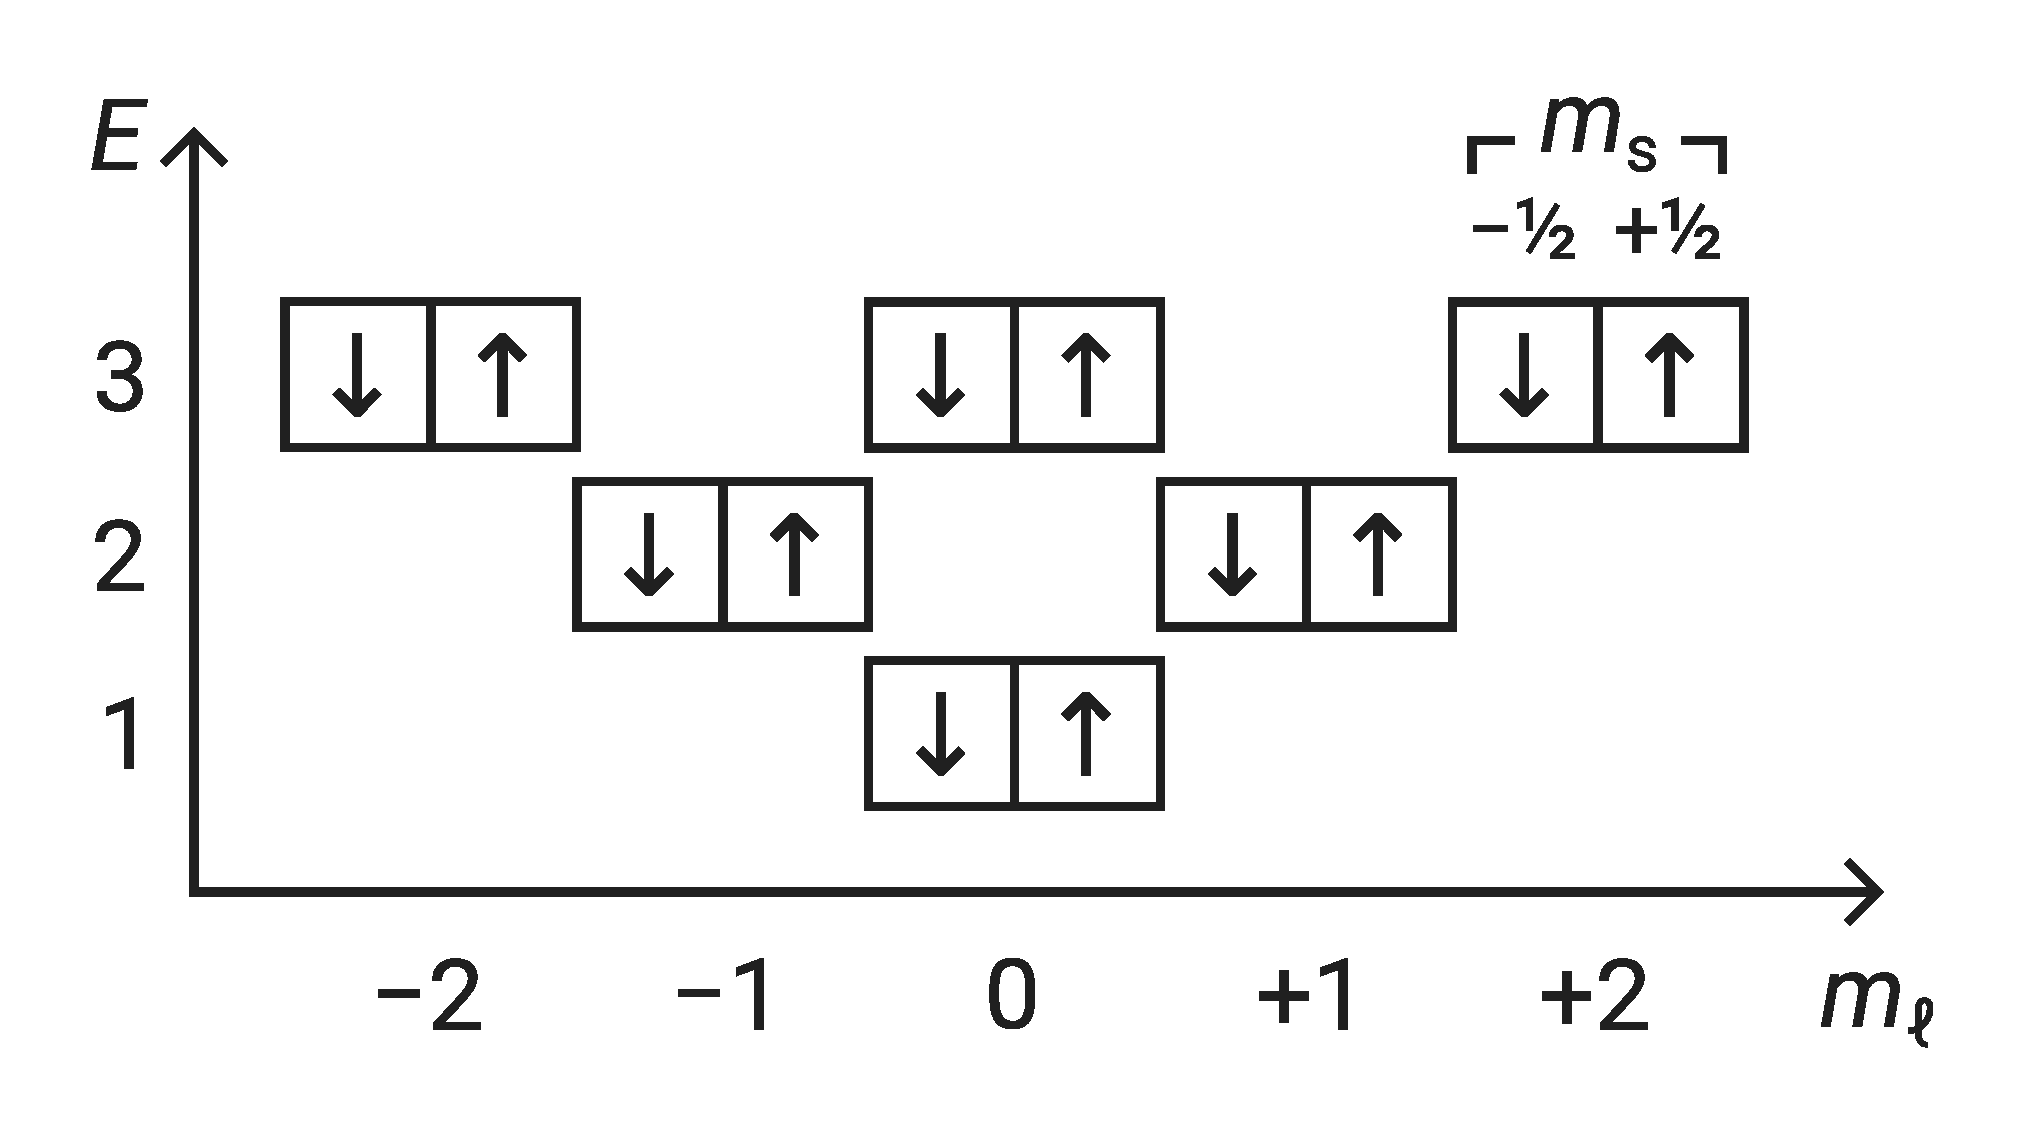
\includegraphics[width=.48\textwidth]{fig-shell-structure}
\caption{Structure of the lowest 12 single-particle states in a noninteracting
  harmonic oscillator of frequency $\omega = 1$.  Each box represents a
  single-particle state, and the arrows denote the spin of the states.}
\label{fig:shell-structure}
\end{figure}
The eigenvalues of the single-particle Hamiltonian $\hat h^{\text o}$ are
given by
\begin{align*}
  \varepsilon_{n, m_\ell, m_{\text s}} \equiv (2 n + |m_\ell| + 1) \omega
\end{align*}
which satisfies
$\hat{h}^{\text o} \ket{\phi_{n, m_\ell, m_{\text s}}} = \varepsilon_{n,
  m_\ell, m_{\text s}} \ket{\phi_{n, m_\ell, m_{\text s}}}$.  Note that the
states are degenerate with respect to the spin projection $m_{\text s}$ since
our Hamiltonian $\hat h^{\text o}$ does not distinguish between them.  From
this equation, we can deduce the shell structure as shown in Figure
\ref{fig:shell-structure}.  It is notable that there are degeneracies beyond
that of the spin pairs: each shell contains a set of states that satisfy the
equation $2 n + |m_\ell| = k$ for some nonnegative integer $k$, which we
conveniently call the \textit{shell index}.  The shells are equidistant from
each other, with a spacing equal to the frequency $\omega$.

The many-body Hamiltonian $\hat H^{\text o}$ is the sum of the single-particle
Hamiltonians $\hat h^{\text o}_p$ over all particles $p$, where $p$ may now be
treated as a tuple of all three single-particle quantum numbers:
$(n, m_\ell, m_{\text s})$.  From the states $\phi$ in
\eqref{eq:singleparticlestate} we can construct the an eigenstate of the
many-body Hamiltonian $\hat H^{\text o}$ in the form of a Slater determinant
$\varnothing_{p_1, \ldots, p_N}$:
\begin{align*}
  \varnothing_{p_1, \ldots, p_N}(\bm r_1, \ldots, \bm r_N) \equiv
  \frac{1}{\sqrt{N}} \left|
  \begin{matrix}
    \phi_{p_1}(\bm r_1) & \cdots & \phi_{p_N}(\bm r_1) \\
    \vdots & \ddots & \vdots \\
    \phi_{p_1}(\bm r_N) & \cdots & \phi_{p_N}(\bm r_N) \\
  \end{matrix}
  \right|
\end{align*}
This automatically satisfies the Pauli exclusion principle, ensuring that the
Fermi statistics are satisfied.  The energy of these states is given by the
sum of the single-particle energies:
\begin{align*}
  E^{\text o}_{p_1, \ldots, p_N} =
  \varepsilon_{p_1} + \cdots + \varepsilon_{p_N},
\end{align*}
which satisfies
$\hat{H}^{\text o} \ket{\varnothing_{p_1, \ldots, p_N}} = E^{\text o}_{p_1, \ldots,
  p_N} \ket{\varnothing_{p_1, \ldots, p_N}}$.  For ground states, we may have
degeneracies due to the shell structure of the single-particle basis.
However, if $N = k_{\text F} (k_{\text F} + 1)$ for some nonnegative integer
$k_{\text F}$, there are just enough particles to form a closed-shell system.
In this case, there is a unique, well-isolated ground state.  The values of
$N$ for which this occurs are typically referred to as \textit{magic numbers}
and we call $k_{\text F}$ the \textit{number of filled shells} (or ``Fermi
level'').  This completes the solution of the noninteracting problem.

The difficulty in solving the full Hamiltonian $\hat H$ stems from the fact
that the exact solution cannot be expressed in terms of a single Slater
determinant due to the presence of interactions.  Hence, it is not possible to
trivially reduce the problem to that of a single particle as we had done
previously.

However, if we assume that the interaction alters the behavior of the system
only mildly, we can use the Slater determinants of the noninteracting system
as an initial guess for the solution, and then apply iterative methods to
improve the accuracy of the solution.

Since Slater determinants are rather cumbersome to write out in full, we shall
instead work in the more convenient formalism of \textit{second quantization}:
\begin{align*}
  \ket{\varnothing_{p_1, \ldots, p_N}} =
  \hat a_{p_1}^\dagger \cdots \hat a_{p_N}^\dagger \ket{\varnothing}
\end{align*}
Here, $\varnothing$ is the vacuum state that is devoid of particles and
$\hat a_p^\dagger$ is a \textit{creation operator} for the single-particle
state $p$.  If the state $p$ is not yet occupied by a particle,
$\hat a_p^\dagger$ creates such a particle.  Otherwise, it collapses the
entire many-body state to $0$.  The Hermitian conjugate of $\hat a_p^\dagger$
is $\hat a_p$, which is an \textit{annihilation operator} for the state $p$
that has the opposite effect.  For fermions, the field operators $\hat a_p$
and $\hat a_p^\dagger$ satisfy the essential anticommutation relations,
\begin{align*}
  &\{\hat a_p, \hat a_q\} = \{\hat a_p^\dagger, \hat a_q^\dagger\} = 0 &
  &\{\hat a_p, \hat a_q^\dagger\} = \delta_{p, q}
\end{align*}
where $\delta_{p, q}$ denotes the Kronecker delta.

Operators can be rewritten in this formalism as well.  The one-body
Hamiltonian $H^{\text o}$ defined by \eqref{eq:onebodyhamiltonian} can be
rewritten in second quantization as
\begin{align} \label{eq:second_quantized_one_body_hamiltonian}
  \hat H^{\text o} = \sum_{p, q} H_{p, q}^{\text o} \hat a_p^\dagger \hat a_q^{}
\end{align}
where the \textit{matrix element}
$H_{p, q}^{\text o} \equiv \bra{\varnothing_p} \hat H^{\text o} \ket{\varnothing_q}$.  This
can likewise be extended to $\hat V$,
\begin{align} \label{eq:second_quantized_two_body_hamiltonian}
  \hat V = \frac{1}{4} \sum_{p, q, r, s} V_{p, q, r, s}^{}
  \hat a_p^\dagger \hat a_q^\dagger \hat a_s^{} \hat a_r^{}
\end{align}
where $U_{p, q} \equiv \langle \varnothing_p | \hat U | \varnothing_q \rangle$ and
$V_{p, q, r, s} \equiv \langle \varnothing_{p, q} | \hat V | \varnothing_{r, s} \rangle$.
The complete Hamiltonian is given by their sum:
\begin{align}
  \hat{H} = \sum_{p, q} H^{\text o}_{p, q} \hat{a}_p^\dagger \hat{a}_q + \frac{1}{4} \sum_{p, q, r, s} V_{p, q, r, s} \hat{a}_p^\dagger \hat{a}_q^\dagger \hat{a}_r \hat{a}_s  \label{eq:vacuumhamiltonian}
\end{align}
Note that due to the antisymmetry present in the Slater determinants, we have
the property that exchanging either $p$ with $q$ or $r$ with $s$ causes
$V_{p, q, r, s}$ to reverse in sign, leading to a $4$-fold symmetry that is
canceled out by the factor of $1/4$.  For this reason, the two-body matrix
element $V_{p, q, r, s}$ is commonly referred to as the \emph{antisymmetrized}
matrix element.  This is not to be confused with the non-antisymmetric
interaction integral defined by:
\begin{align*}
  \tilde V_{p, q, r, s} \equiv \int \phi_p(\bm r) \phi_q(\bm r') v(\bm r, \bm r') \phi_r(\bm r) \phi_s(\bm r') \D \bm r \D \bm r'
\end{align*}
The antisymmetrized matrix element is computed from the interaction integral
by $V_{p, q, r, s} = \tilde V_{p, q, r, s} - \tilde V_{p, q, s, r}$.  In our
work, we compute the interaction numerically via the OpenFCI software, which
numerical integrates the Coulomb interaction in the center-of-mass frame
[[cite Kvaal's paper; also, is the description correct?]].

There are significant advantages in the second quantization formalism in
many-body theory: the operators are written in a way that does not generic
with respect to the number of particles, and the anticommutative behavior of
field operators ensures the Pauli exclusion principle holds no matter how the
operator is manipulated.  Furthermore, it allows the application of a useful
combinatoric theorem known as Wick's theorem [[cite something]] to simplify
complicated operator expressions.  Ultimately, the computations themselves do
not involve operators at all -- rather, they involve the calculation of
\emph{matrix elements} via equations derived with the aid of Wick's theorem.

\subsection{Hartree-Fock method}
\label{subsec:HartreeFockmethod}

The first correction that we will apply to our solution is that of the
Hartree-Fock (HF) method.  Using the variational principle, we compute an
approximate ground state $\Phi$ by minimizing the energy expectation value
\begin{align*}
  E_{\Phi} \equiv \langle \Phi | \hat H | \Phi \rangle
\end{align*}
with respect to $\Phi$, subject to the restriction that
$\Phi$ is a single Slater determinant constructed from an unknown
set of $N$ orthonormal single-particle states.  We denote each unknown
single-particle state $\phi_{q}'$ by some label $q$.

To make this computationally feasible, we further assume that the unknown
states $\{\phi_q'\}$ are built from a linear combination of known functions,
drawn from a finite set $\{\phi_p\}$.  This reduces the problem from an
abstract mathematical one to a numerical linear algebra problem, with the
caveat that this set of known functions must be chosen carefully to ensure
convergence.

Assuming the interaction is not too strong, we can use the single-particle
states $\{\phi_p\}$ of our noninteracting Hamiltonian as a basis for the
unknown states $\{\phi'_u\}$.  The two sets of states are then related by a
linear transformation matrix $\bm C$:
\begin{align*}
  \phi_q' \equiv \sum_p \phi_p C_{p, q}
\end{align*}
To ensure the orthonormality of the states, we assume the set of unknown states $\{\phi_q'\}$ has as many elements as the set of $\{\phi_p\}$ and require the coefficient matrix $\bm C$ to be unitary.  While these conditions are more strict than necessary, they greatly simplify the calculations and allow the states $\{\phi_q'\}$ to act as inputs for methods beyond HF.  The set of states $\{\phi_q'\}$ now consists of $N$ \textit{occupied} states that participate in the Slater determinant $\Phi$ and the remaining \textit{unoccupied} states that do not.

Since the coefficient matrix uniquely determines the unknown states, the variational problem has been reduced to that of solving of the coefficients $\bm C$ that minimize the energy $E_{\Phi}$, which is given by
\begin{align}
  E_{\Phi} &= \sum_{j} n_j H^{\text{o} \prime}_{j, j} + \sum_{j, k} n_j n_k V'_{j, k, j, k} \label{eq:hfenergy}
\end{align}
where the transformed operators are defined as
\begin{align}
  H^{\text{o} \prime}_{p, q} &\equiv \sum_{r, s} C_{r, p}^* H_{r, s}^{\text o} C_{s, q}^{} \label{eq:hftransform1} \\
  V'_{p, q, r, s} &\equiv \sum_{t, u, v, w} C_{t, p}^* C_{u, q}^* V_{t, u, v, w}^{} C_{v, r}^{} C_{w, s}^{} \label{eq:hftransform2}
\end{align}
and the occupancy number $n_p$ is defined as
\begin{align}
  n_p \equiv \begin{cases}
    1 & \text{if $p$ is an occupied state in $\Phi$} \\
    0 & \text{if $p$ is an unoccupied state in $\Phi$}
  \end{cases}
\end{align}
and further define $\bar n_p \equiv 1 - n_p$ as the complement.

With the method of Lagrange multipliers, the minimization problem can be reduced to the solving of a nonlinear equation -- the \textit{Hartree-Fock equation}:
\begin{align} \label{eq:hartreefock}
  \bm F \bm C = \bm C \bm \epsilon
\end{align}
where the \textit{Fock matrix} $\bm F$ is defined as
\begin{align} \label{eq:fock}
  F_{p, q} \equiv H_{p, q}^{\text o} + \sum_{r, s, j} n_j C_{r, j}^* V_{p, r, q, s}^{} C_{s, j}^{}
\end{align}
and $\bm \epsilon$ is a vector of Lagrange multipliers with each element $\epsilon_q$ associated with a particular state $\phi'_q$.

The HF equation can be solved by an iterative technique: a solution $\bm C$ can be fed into \eqref{eq:fock} and new solution can then obtained by solving the eigenvalue problem in \eqref{eq:hartreefock} using the Fock matrix obtained.  For the initial guess, we use the ground state of our noninteracting Hamiltonian, thus $\bm C$ is initially the identity matrix.  After dozens of iterations, perhaps with the aid of a convergence acceleration technique (such as DIIS [[cite??] or Broyden's method [[cite?]]), one would usually reach a state of self-consistency where the solution converges to a fixed value.  This is the Hartree-Fock solution.

Since HF restricts the ground state to a Slater determinant of single-particle
states, it cannot provide an exact solution to a problem where correlations
are present even if the basis $\{\phi_p\}$ is not truncated (infinite).  The
energy difference between the best Hartree-Fock energy and the exact ground
state energy is thus by definition known as the \textit{correlation energy}.
The focus of post-HF methods such as IM-SRG is to improve on the HF results,
thus recovering parts of this missing energy.

To make use of the HF solution as the reference state for future calculations, we transform the operators via \eqref{eq:hftransform1} and \eqref{eq:hftransform2}.  Therefore, the post-HF methods described in the next few sections generally use the transformed operators $\hat H^{\text{o} \prime}$ and $\hat V'$ as inputs.  However, for generality, we omit the prime symbols as the methods do not necessitate a state optimized by HF.

\subsection{The IM-SRG method}
\label{subsec:imsrgmethod}

\subsubsection{Similarity renormalization group methods}
\label{subsubsec:srgmethods}

In similarity renormalization group (SRG) methods, one performs a continuous
sequence of unitary transformations on a Hamiltonian operator $\hat H$ to
evolve it into a band- or block-diagonal form, reducing the coupling between a
small model space of interest from its complementary space.  This allows the
Hilbert space to be truncated to the small model space without losing
significant accuracy.

The sequence of transformations is parameterized by a continuous variable $s$
known as the \textit{flow parameter}.  By convention we define to be $0$ at
the beginning of the sequence, and thus the evolving Hamiltonian $\hat H(s)$
at $s = 0$ is set to the original Hamiltonian.  Upon reaching $s$, the
transformed Hamiltonian is given by
\begin{align*}
  \hat H(s) \equiv \hat U(s) \hat H(0) \hat U^\dagger(s)
\end{align*}
where $U(s)$ is a unitary operator that describes the product of all such
transformations since $s = 0$.  Taking the derivative with respect to $s$, we obtain:
\begin{align*}
  \frac{\D}{\D s} H(s) =
  \left(\frac{\D}{\D s} \hat{U}(s)\right) \hat{H}(0) \hat{U}^\dagger(s) +
  \hat{U}(s) \hat{H}(0) \frac{\D}{\D s} \hat{U}^\dagger(s)
\end{align*}
If we define an operator $\eta(s)$ as
\begin{align*}
  \eta(s) \equiv \left(\frac{\D}{\D s} \hat{U}(s)\right) \hat{U}^\dagger(s)
\end{align*}
we find that it is antihermitian as a result of the unitarity of $\hat{U}(s)$:
\begin{align*}
  \eta(s) + \eta^\dagger(s)
  = \frac{\D}{\D s} \left(\hat{U}(s) \hat{U}^\dagger(s)\right)
  = 0
\end{align*}
From this property we can derive a differential equation known as the
\textit{SRG flow equation}:
\begin{align} \label{eq:imsrgode}
  \frac{\D}{\D s} H(s) = [\eta(s), \hat{H}(s)]
\end{align}
The equation allows $\hat{H}(s)$ to be evaluated without explicitly
constructing the full transformation $\hat U(s)$.  The operator $\hat \eta(s)$
is known as the \textit{generator} of the transformation.  When ``integrated''
as a product, the full transformation $\hat U(s)$ is recovered:
\begin{align*}
  \hat U(s')
  = \mathcal T_s \left\{ \mathrm{e}^{\int_0^{s'} \hat{\eta}(s) \D s} \right\}
  \equiv \lim_{\Delta s \to 0} \prod_{s = 0, \Delta s, \ldots}^{s = s'}
  \mathrm{e}^{\hat \eta(s) \Delta s}
\end{align*}
Here $\mathcal T_s$ is a notational device that denotes $s$-ordering: a reordering of the $\hat{\eta}(s)$ operator products expanded from the exponential with respect to $s$ in ascending order \cite[\S 6.1]{reimann2013quantum}.  This is analogous to the usual time-ordering from quantum field theory.

The operator $\hat{\eta}$ can be chosen to suppress certain undesirable parts of the Hamiltonian matrix, which can be considered the ``off-diagonal'' parts in a loose sense.  The ``off-diagonal'' parts could be elements far away from the matrix diagonal, in which case the evolution drives the matrix towards a band-diagonal form.  Or, the ``off-diagonal'' parts could be elements that couple the ground state from the excited state, in which case the evolution drives the matrix towards a block-diagonal form that isolates the ground state.  Or, the ``off-diagonal'' could be literally the elements that do not lie on the diagonal, in which case the evolution would simply diagonalize the Hamiltonian.  Through different choices of $\hat{\eta}$, the SRG evolution can be controlled and adapted to the features of a particular problem.

\subsubsection{Evolving the flow equation in medium}

The SRG flow equation \eqref{eq:imsrgode} can be solved in the second quantization formalism described in Section \ref{subsec:modelHamiltonian}, where field operators are defined with respect to the physical vacuum state.  However, since the size of the problem grows enormously with the number of particles and the size of the model space, the applicability of this free-space SRG method is restricted to comparatively small systems.  Alternatively, the evolution can be done at finite density, i.e.\ directly in an $N$-particle system defined by a reference state \cite{kehrein2006flow}.  This gives rise to the IM-SRG method.

The second-quantized operators in \eqref{eq:second_quantized_one_body_hamiltonian} and \eqref{eq:second_quantized_two_body_hamiltonian} are constructed with respect to the vacuum state.  That is, the operator strings $\hat{a}_p^\dagger \hat{a}_q$ and $\hat{a}_p^\dagger \hat{a}_q^\dagger \hat{a}_s \hat{a}_r$ both have a vacuum expectation value of zero:
\begin{align*}
&\bra{\varnothing} \hat{a}_p^\dagger \hat{a}_q \ket{\varnothing} = 0 &
&\bra{\varnothing} \hat{a}_p^\dagger \hat{a}_q^\dagger \hat{a}_s \hat{a}_r \ket{\varnothing} = 0
\end{align*}
They are said to be \emph{normal-ordered} with respect to the vacuum state $\varnothing$.  It is possible to be normal-ordered with respect to a non-vacuum state, however.  Consider a Slater determinant $\Phi$ with $N_{\text F}$ occupied states:
\begin{align*}
  \ket{\Phi} \equiv \ket{\varnothing_{i_1, i_2, \ldots, i_{N_{\text F}}}}
\end{align*}
where $\{i_1, i_2, \ldots, i_{N_{\text F}}\}$ is a set of $N_{\text F}$ indices that label the occupied states.  One can define a set of \textit{quasiparticle field operators} $\hat b$ and $\hat b^\dagger$ that obey the same anticommutation relations as the $\hat a$ operators:
\begin{align*}
  \hat b_p \equiv \bar n_p \hat a_{p} + n_p \hat a_{p}^\dagger
\end{align*}
The quasiparticle field operators treat $\ket{\Phi}$ as their ``vacuum state'' (sometimes called ``Fermi vaccuum'' in an abstract sense), despite not being the physical vacuum state.  As before, it is possible to construct arbitrary Slater determinants by applying quasiparticle operators to the reference state:
\begin{align}
  \ket{\Phi_{p_1, \ldots, p_k}} \equiv \hat{b}^\dagger_{p_1} \cdots \hat{b}^\dagger_{p_k} \ket{\Phi}
  \label{eq:quasisd}
\end{align}
In nonrelativistic many-body theory, it is expected that $\{p_1, \ldots, p_k\}$ contain a balanced number of occupied and unoccupied states to conserve the total number of particles; otherwise, the Slater determinant would represent a different system.

We may then define \emph{normal ordering with respect to the reference state} $\Phi$, a notational device that rearranges a string of operators such that every quasiparticle creation operator appears before a quasiparticle annihilation operator by repeatedly exchanging neighboring operators, with each exchange incurring a change in sign.  A simple example would be the normal ordering of a pair of field operators such as:
\begin{align*}
  \normord{\hat{b}_p \hat{b}_q^\dagger} =
  -\hat{b}_q^\dagger \hat{b}_p
\end{align*}
Here, we denote normal ordering of an operator string with respect to $\Phi$ by a pair of colons.  The expectation value of a normal ordered string of operators with respect to $\Phi$ is guaranteed to vanish:
\begin{align*}
&\bra{\Phi} \hat{b}_p^\dagger \hat{b}_q \ket{\Phi} = 0 &
&\bra{\Phi} \hat{b}_p^\dagger \hat{b}_q^\dagger \hat{b}_s \hat{b}_r \ket{\Phi} = 0
\end{align*}
The normal ordering of the quasiparticle field operators are straightforward to compute, but what is more interesting is the normal ordering of the physical field operators $\hat a$ and $\hat a^\dagger$ with respect to $\Phi$:
\begin{align*}
  \normord{\hat{a}_p^\dagger \hat{a}_q} &=
  \hat{a}_p^\dagger \hat{a}_q - n_p \delta_{p, q}
\end{align*}
The normal ordering notation thus provides a concise way of expressing the right-hand side.  In this new notation, we can rewrite the Hamiltonian $\hat H = \hat H^{\text o} + \hat V$ in its \emph{normal-ordered representation}:
\begin{align}
  \hat{H} = H^{[0]} + \sum_{p, q} H^{[1]}_{p, q} \normord{\hat{a}_p^\dagger \hat{a}_q} + \frac{1}{4} \sum_{p, q, r, s} H^{[2]}_{p, q, r, s} \normord{\hat{a}_p^\dagger \hat{a}_q^\dagger \hat{a}_r \hat{a}_s}
  \label{eq:normordhamiltonian}
\end{align}
where
\begin{align*}
  H^{[0]} &\equiv \sum_{i} n_i H^{\text o}_{i, i} + \frac{1}{2} \sum_{i, j} n_i n_j V_{i, j, i, j} \\
  H^{[1]}_{p, q} &\equiv H^{\text o}_{p, q} + \sum_{i} n_i V_{p, i, q, i} \\
  H^{[2]}_{p, q, r, s} &\equiv V_{p, q, r, s} \\
\end{align*}
If $\Phi$ is a state optimized by the HF method, then $H^{[0]}$ is simply the HF energy $E_\Phi$ and $H^{[1]}_{p, q}$ is the Fock matrix $F_{p, q}$.  The normal-ordered representation of $\hat H$ in \eqref{eq:normordhamiltonian} is completely equivalent to that of $\hat H$ in \eqref{eq:vacuumhamiltonian}.  The only difference is that it rearranges the matrix elements so as to emphasize the reference state $\Phi$ rather than vacuum state $\ket{\varnothing}$.  This makes a critical difference when the expressions containing 3-body or higher terms are \emph{truncated} to only 2-body.  If the reference state $\Phi$ is good approximation of the true solution $\Psi$, then the importance of the higher-body parts of the Hamiltonian are greatly reduced.

Higher-body operators arise from integrating the flow equations (\ref{eq:imsrgode}), which is one of the major challenges of the SRG method.  With each evaluation of the commutator, the Hamiltonian gains terms of higher order, and these induced contributions will in subsequent integration steps feed back into terms of lower order.  Thus, the higher-body contributions are not irrelevant to the final solution even if only the ground state energy is of interest.

Computationally, higher-body terms are difficult to handle: the amount of memory required to store an $r$-body operator is grows exponentially with $r$.  Moreover, the flow equations are capable of generating an infinite number of higher-body terms as the Hamiltonian evolves.  Thus, to make the method tractable, we must close the IM-SRG flow equations, truncating the equations to a finite order.

In this paper, we truncate both $\hat{H}$ and $\hat{\eta}$ at the two-body level, an approach known as IM-SRG(2).  This normal-ordered two-body approximation appears to be sufficient in many cases and has yielded excellent results for several nuclei \cite{PhysRevLett.106.222502,PhysRevLett.109.052501,IMSRG}.

Note that the loss of three-body and higher-body terms (\textit{operator truncation}) is only one out of the two sources of error in this method.  The other source of error is due to the \textit{basis truncation}, as with any method that relies on a finite single-particle basis.  The latter can be reduced by increasing the size of the basis at the expense of greater computational effort.

With the operator truncation, the generator $\hat{\eta}$ can be written as a generic antihermitian 2-body operator:
\begin{align*}
\hat{\eta} = \sum_{p, q} \eta_{p, q}^{[1]} \normord{\hat a_p^\dagger \hat a_q} +
\frac{1}{4} \sum_{p, q, r, s}\eta_{p, q, r, s}^{[2]} \normord{\hat a_p^\dagger \hat a_q^\dagger \hat a_s \hat a_r}
\end{align*}
where $\eta_{p, q}^{[1]}$ and $ \eta_{p, q, r, s}^{[2]}$ respectively are its one- and two-body matrix elements normal ordered with respect to $\Phi$.

By expanding the commutator in \eqref{eq:imsrgode} without consideration of the three-body term, we obtain the matrix-element form of the IM-SRG(2) flow equation:
\begin{align}
    \frac{\D H^{[r]}}{\D s} = C^{[r]}(\eta, H) \label{eq:flowmxe}
\end{align}
where
\begin{align}
  C^{[r]}(A, B) &\equiv \tilde{\mathcal{A}}_{A, B} D^{[r]}(A, B) \text{ for any $r$, $A$, $B$} \label{eq:commutmxe} \\
  \tilde{\mathcal{A}}_{x, y} f(x, y) &\equiv f(x, y) - f(y, x) \text{ for any $x$, $y$, $f$}
\end{align}
and finally
\begin{widetext}
  \begin{align}
    D^{[0]}(A, B)
    &\equiv
      \sum_{i, a} n_i \bar{n}_a A^{[1]}_{i, a} B^{[1]}_{a, i}
      + \frac{1}{4} \sum_{i, j, a, b} n_i n_j \bar{n}_a \bar{n}_b A^{[2]}_{i, j, a, b} B^{[2]}_{a, b, i, j}
      \label{eq:flow0} \\
    D^{[1]}_{p, q}(A, B)
    &\equiv
      \sum_{r} A^{[1]}_{p, r} B^{[1]}_{r, q}
      - \frac{1}{2} \sum_{i, j, a} n_i n_j \bar{n}_a A^{[2]}_{i, j, a, q} B^{[2]}_{a, p, i, j}
      + \frac{1}{2} \sum_{i, a, b} n_i \bar{n}_a \bar{n}_b A^{[2]}_{i, p, a, b} B^{[2]}_{a, b, i, q}
      \notag \\
    &\hphantom{=}
      + \sum_{i, a} n_i \bar{n}_a \left(
        A^{[1]}_{i, a} B^{[2]}_{a, p, i, q}
        + A^{[2]}_{i, p, a, q} B^{[1]}_{a, i}
      \right)
      \label{eq:flow1} \\
    D^{[2]}_{p, q, r, s}(A, B)
    &\equiv
      \tilde{\mathcal{A}}_{p, q} \tilde{\mathcal{A}}_{r, s}
        \sum_{i, a} n_i \bar{n}_a A^{[2]}_{i, p, a, r} B^{[2]}_{a, q, i, s}
      + \frac{1}{2} \sum_{i, j} n_i n_j A^{[2]}_{i, j, r, s} B^{[2]}_{p, q, i, j}
      + \frac{1}{2} \sum_{a, b} \bar{n}_a \bar{n}_b A^{[2]}_{p, q, a, b} B^{[2]}_{a, b, r, s}
      \notag \\
    &\hphantom{=}
      + \sum_{t} \left(
        \tilde{\mathcal{A}}_{p, q} A^{[1]}_{q, t} B^{[2]}_{p, t, r, s}
        + \tilde{\mathcal{A}}_{r, s} A^{[2]}_{p, q, r, t} B^{[1]}_{t, s}
      \right)
      \label{eq:flow2}
\end{align}
\end{widetext}
\begin{figure}
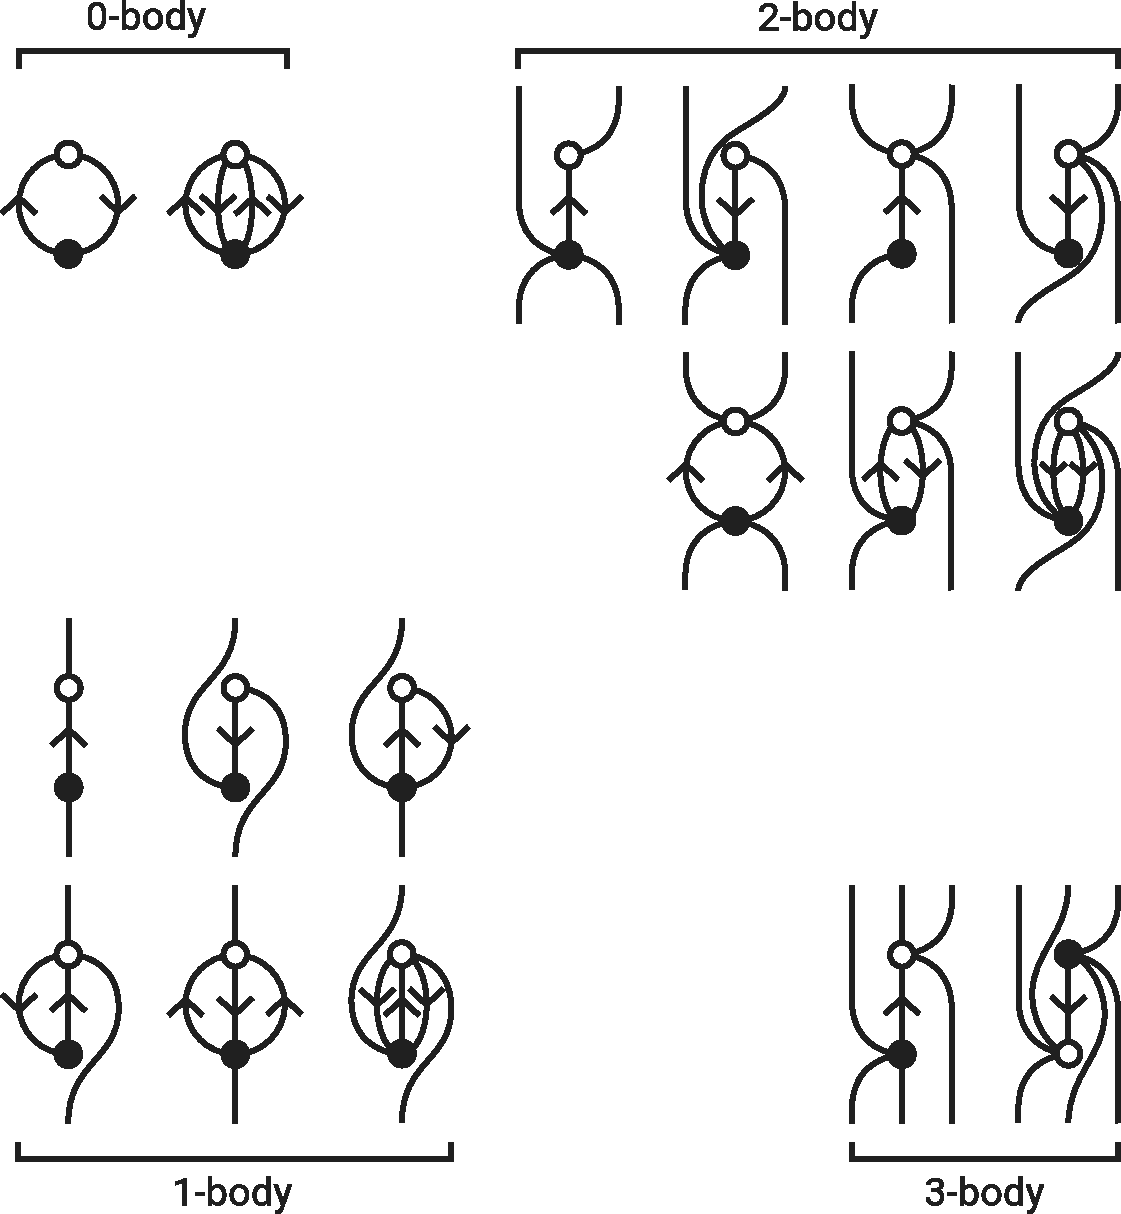
\includegraphics[width=.48\textwidth]{fig-diagrams-imsrg}
\caption{Diagrammatic representation of $C^{[r]}(\circ, \bullet)$ in \eqref{eq:commutmxe} that forms part of the IM-SRG flow equation \eqref{eq:flowmxe}.  The diagrams are implicitly antisymmetrized (Hugenholtz diagrams \cite{HUGENHOLTZ1957481} as described in \cite{shavitt2009many} \S 4.4.3).}
\label{fig:diagrams-imsrg}
\end{figure}
The equations can be derived directly from the anticommutation relations of the field operators, but it is more convenient to use Wick's theorem [[ref]] or, even more efficiently, diagrammatic techniques [[ref]] to arrive at the results.  In particular, the diagrammatic representation of antisymmetrized matrix elements are shown in Figure \ref{fig:diagrams-imsrg}.

An accurate and robust ODE solver is required to solve \eqref{eq:imsrgode}.  In particular, the solver must be able to handle the stiffness that can often arise (even in the case of White generator).  For this, we use an accurate, high-order ODE solver implementation by Shampine and Gordon that uses the Adams predictor-corrector formulas [[Ref: Shampine and Gordon book]].

Through the flow equation and with an appropriate choice of the generator $\hat{\eta}$, the evolved state $\hat U(s) \ket{\Phi}$ will gradually approach a more ``diagonal'' form.  If the ``diagonal'' form decouples the ground state from the excited states, then $\hat U(\infty) \ket{\Phi}$ would yield the exact ground state solution of the problem if no operator or basis truncations are made.  In particular, $H^{[0]}$ would approach the true ground state energy.

The commutator in the flow equations \eqref{eq:imsrgode} guarantees that the evolved state $\hat U(s) \ket{\Phi}$ can be expanded in terms of \emph{linked diagrams} only \cite{shavitt2009many,ISI:A1981MN73700014}, which demonstrates that IM-SRG is size-extensive.  Regarding the quality of the SRG results, it means that the error introduced by truncating the many-body expansions scales linearly with the number of particles $N$.

\subsubsection{Wegner's canonical generator}

To determine the specific unitary transformation, one needs to specify the generator $\hat{\eta}$.  Through different choices, the SRG flow can be adapted to the features of a particular problem.

The original choice suggested by Wegner \cite{PhysRepWegner0} reads
\begin{equation}
  \hat{\eta}_{\text{Wegner}}
  = [\hat{H}^{\text{d}}, \hat{H} - \hat{H}^{\text{d}}]
  = [\hat{H}^{\text{d}}, \hat{H}]
  \label{eq:etaWegner}
\end{equation}
where $\hat{H}^{\text{d}}$ denotes the ``diagonal'' part of the Hamiltonian (and $\hat{H} - \hat{H}^{\text{d}}$ denotes the ``off-diagonal'' part) in the abstract sense described at the end of section \ref{subsubsec:srgmethods}.

The commutator between two Hermitian operators, $\hat{\eta}$ is always antihermitian, as required for a generator.  Additionally, it can be shown that the commutator has the property of suppressing off-diagonal matrix elements as the state evolves via the flow equation \cite{kehrein2006flow}, as we would like.  In particular, matrix elements far off the diagonal, where the Hamiltonian couples states with large energy differences, are suppressed much faster than elements closer to the diagonal.

The matrix elements of the generator can be evaluated using \eqref{eq:commutmxe} to \eqref{eq:flow2}.  If assume that $\hat{H}^{\text{d}}$ does not couple the ground state to the excited states, the equations can be simplified considerably: [[clean up this equation]]
\begin{align*}
\eta_{pq}^{(1)} = & \sum_{r} \left(f_{pr}^d f_{rq} - f_{pr} f_{rq}^d \right) + f_{pq} v_{qppq}^d \left( n_q - n_p \right) \\ \eta_{pqrs}^{(2)} = & - \sum_t \left\lbrace \tilde{\mathcal{A}}_{p, q} f_{pt} v_{tqrs}^d - \tilde{\mathcal{A}}_{r, s} f_{tr} v_{pqts}^d \right\rbrace \notag \\ & + \sum_t \left\lbrace \tilde{\mathcal{A}}_{p, q} f_{pt}^d v_{tqrs} - \tilde{\mathcal{A}}_{r, s} f_{tr}^d v_{pqts} \right\rbrace \notag \\ & + \frac{1}{2} \sum_{tu} (1 - n_t - n_u) \left( v_{pqtu}^d v_{turs} - v_{pqtu} v_{turs}^d \right) \notag \\ & + \sum_{tu} \left( n_t - n_u \right) \tilde{\mathcal{A}}_{p, q} \tilde{\mathcal{A}}_{r, s} v_{tpur}^d v_{uqts},
\end{align*}

\subsubsection{White's generator}

Apart from Wegner's choice of the generator, there exist several other ones in literature. One choice, proposed by White \cite{White:cond-mat0201346}, makes numerical approaches much more efficient.  The problem with Wegner's generator is the widely varying decaying speeds of the Hamiltonian matrix elements.  Terms with large energy separations from the ground state are suppressed initially, followed by those with smaller energy separations.  This leads to stiffness in the flow equation, leading to numerical difficulties in solving the set of coupled differential equations.

White takes an alternative approach, which is especially suited for problems where one is interested in the ground state of a system.  Firstly, instead of driving all off-diagonal elements of the Hamiltonian to zero, he focuses solely on those ones that are connected to the reference state $\Phi$, aiming to decouple the reference state from the remaining Hamiltonian.  This reduces the amount of change performed on the Hamiltonian, which can reduce the accuracy loss resulting from the truncated higher-body terms.  Secondly, the rate of decay in Hamiltonian matrix elements are approximately normalized by dividing the generator matrix elements by an appropriate factor.  This reduces the stiffness of the flow equations.

The generator is explicitly constructed the following way \cite{PhysRevLett.106.222502,White:cond-mat0201346}
\begin{align}
\hat{\eta}_{\text{White}} &\equiv \hat{\eta}' - \hat{\eta}'{}^\dagger
\end{align}
where
\begin{align}
\eta^{\prime [1]}_{a, i} &\equiv \frac{\bar{n}_a n_i H^{[1]}_{a, i}}{H^{[1]}_{a, a} - H^{[1]}_{i, i} - H^{[2]}_{a, i, a, i}}
\label{eq:WhiteFull1} \\
\eta^{\prime [2]}_{a, b, i, j} &\equiv \frac{4 \bar{n}_a \bar{n}_b n_i n_j H^{[2]}_{a, b, i, j}}{H^{[1]}_{a, a} + H^{[1]}_{b, b} - H^{[1]}_{i, i} - H^{[1]}_{j, j} + X_{a, b, i, j}}
\label{eq:WhiteFull2} \\
X_{a, b, i, j}
  &\equiv v_{a, b, a, b} + v_{i, j, i, j} \notag \\
  &\hphantom{\equiv} - v_{a, i, a, i} - v_{a, j, a, j} \notag \\
  &\hphantom{\equiv} - v_{b, i, b, i} - v_{b, j, b, j}
\label{eq:White7}
\end{align}

Compared to Wegner's canonical generator, where the final flow equations involve cubes of the one-body and two-body Hamiltonian matrix elements, these elements contribute only linearly with White's generator, which results in much better numerical properties.  [[It is not explained at all what ``final flow equations'' means]]

\subsection{Quasigenerate perturbation theory}
\label{subsec:selfenergy}

IM-SRG, in the approach described, provides a means to calculate the ground state energy of any system that is reasonably approximated by a single Slater determinant.  This works well for closed-shell systems, but it does not provide a direct means to obtain the ground state energy of open-shell systems.  While there exists more complicated multi-reference approaches to IM-SRG that can tackle the general problem \cite{Hergert2016165}, we opted to use the simpler quasidegenerate perturbation theory (QDPT), which provides us with a simple approach to extract ground state energies of open-shell systems that are only a few particles removed from a closed-shell system.  In particular, it allows us to calculate \textit{addition energies} $\epsilon_a$ and \textit{removal energies} $\epsilon_i$ of such systems, which we define as:
\begin{align}
  \epsilon_a &\equiv E_{\Phi_a} - E_{\Phi} \\
  \epsilon_i &\equiv E_{\Phi} - E_{\Phi_i}
\end{align}
where the meaning of $\Phi_p$ is defined in \eqref{eq:quasisd}, $i$ is restricted to labels of occupied states, and $a$ is restricted to labels of unoccupied states.

In QDPT, the solutions of the approximate Hamiltonian $\hat H^{\text o}$ are used as the basis of the model space.  One then assumes the existence of an operator $\hat \Omega$, known as the \textit{wave operator}, that maps some set of states $\tilde \Psi^{\text o}_u$ within the model space to the exact ground state $\Psi_u$:
\begin{align} \label{eq:omega-condition1}
  \Psi_u = \hat \Omega \tilde \Psi^{\text o}_u
\end{align}
The states $\tilde \Psi^{\text o}_u$ consist of some mixture of the eigenstates
$\Psi^{\text o}_{u'}$ of the approximate Hamiltonian $\hat H^{\text o}$.

There is some freedom in the choice of the wave operator $\hat \Omega$.  We
assume it has the following form:
\begin{align} \label{eq:omega-condition2}
  \hat \Omega = \hat P + \hat Q \hat \Omega \hat P
\end{align}
where $\hat P$ projects any state into the model space and $\hat Q$ is the
complement of $\hat P$.  This entails that the exact states $\Psi_u$ is no
longer normalized but instead satisfies the typical intermediate
normalization: $\langle \Psi_u | \tilde \Psi^{\text o}_u \rangle = 1$.

Making use of the assumptions in Eq.\ \eqref{eq:omega-condition1} and \eqref{eq:omega-condition2}, one can derive from the Schr\"odinger equation the generalized Bloch equation, the principal equation of QDPT:
\begin{gather*}
  [\hat \Omega, \hat H^{\text o}] =
  (1 - \hat \Omega) \hat V \Omega
\end{gather*}
where $\hat V \equiv \hat H - \hat H^{\text o}$ is the perturbation.  The
commutator on the left may be ``inverted'' using the resolvent approach
(\cite{shavitt2009many}, p.\ 50), resulting in:
\begin{align*}
  \hat Q \Omega \hat P_u =
  \hat R_u (1 - \hat \Omega) \hat V \Omega \hat P_u
\end{align*}
where $\hat R_u \equiv \hat Q (E_u - \hat Q \hat H^{\text o} \hat Q)^{-1} \hat Q$ is the resolvent and $\hat P_u$ is the projection operator that projects any state onto $\Psi^{\text o}_u$.  As is typical in perturbation theory, we assume $\hat \Omega$ can be expanded as a series of the increasing order as measured by the ``power'' of the perturbation $\hat V$:
\begin{align*}
  \hat \Omega = \hat P +
  \hat Q\bigl(\hat \Omega_1 + \hat \Omega_2 + \cdots\bigr) \hat P
\end{align*}
This leads to a recursion relation of $\hat \Omega$ that enables $\hat \Omega$ to be calculated up to any order, as least in principle.  Up to third order, we have: [[double-check]]
\begin{align*}
  &\hat \Omega_1 \hat P_u = \hat R_u \hat V \hat P_u \\
  &\hat \Omega_2 \hat P_u =
    \hat R_u \biggl(
    \hat V \hat R_u
    - \sum_v \hat R_v \hat V \hat P_v
    \biggr) \hat V \hat P_u \\
  &\hat \Omega_3 \hat P_u =
    \hat R_u \biggl(
    \hat V \hat R_u \hat V \hat R_u
    - \hat V \hat R_u \sum_v \hat R_v \hat V \hat P_v \\
  &\qquad\qquad
    - \sum_v \hat R_v \hat V \hat P_v \hat V \hat R_u
    - \sum_v \hat R_v \hat V \hat R_v \hat V \hat P_v \\
  &\qquad\qquad
    + \sum_v \hat R_v \sum_w \hat R_w \hat V \hat P_w \hat V \hat P_v
    \biggr) \hat V \hat P_u
\end{align*}
Until now, the solution is described purely in terms of abstract operators in Hilbert space.  To make this concrete and relevant for many-body physics, we must make some additional assumptions.  First, we make use of the single-particle basis as we have for HF and IM-SRG.  Secondly, we assume the set of reference states $\Psi^{\text o}_u$ are Slater determinants of the single-particle states.

\begin{figure}
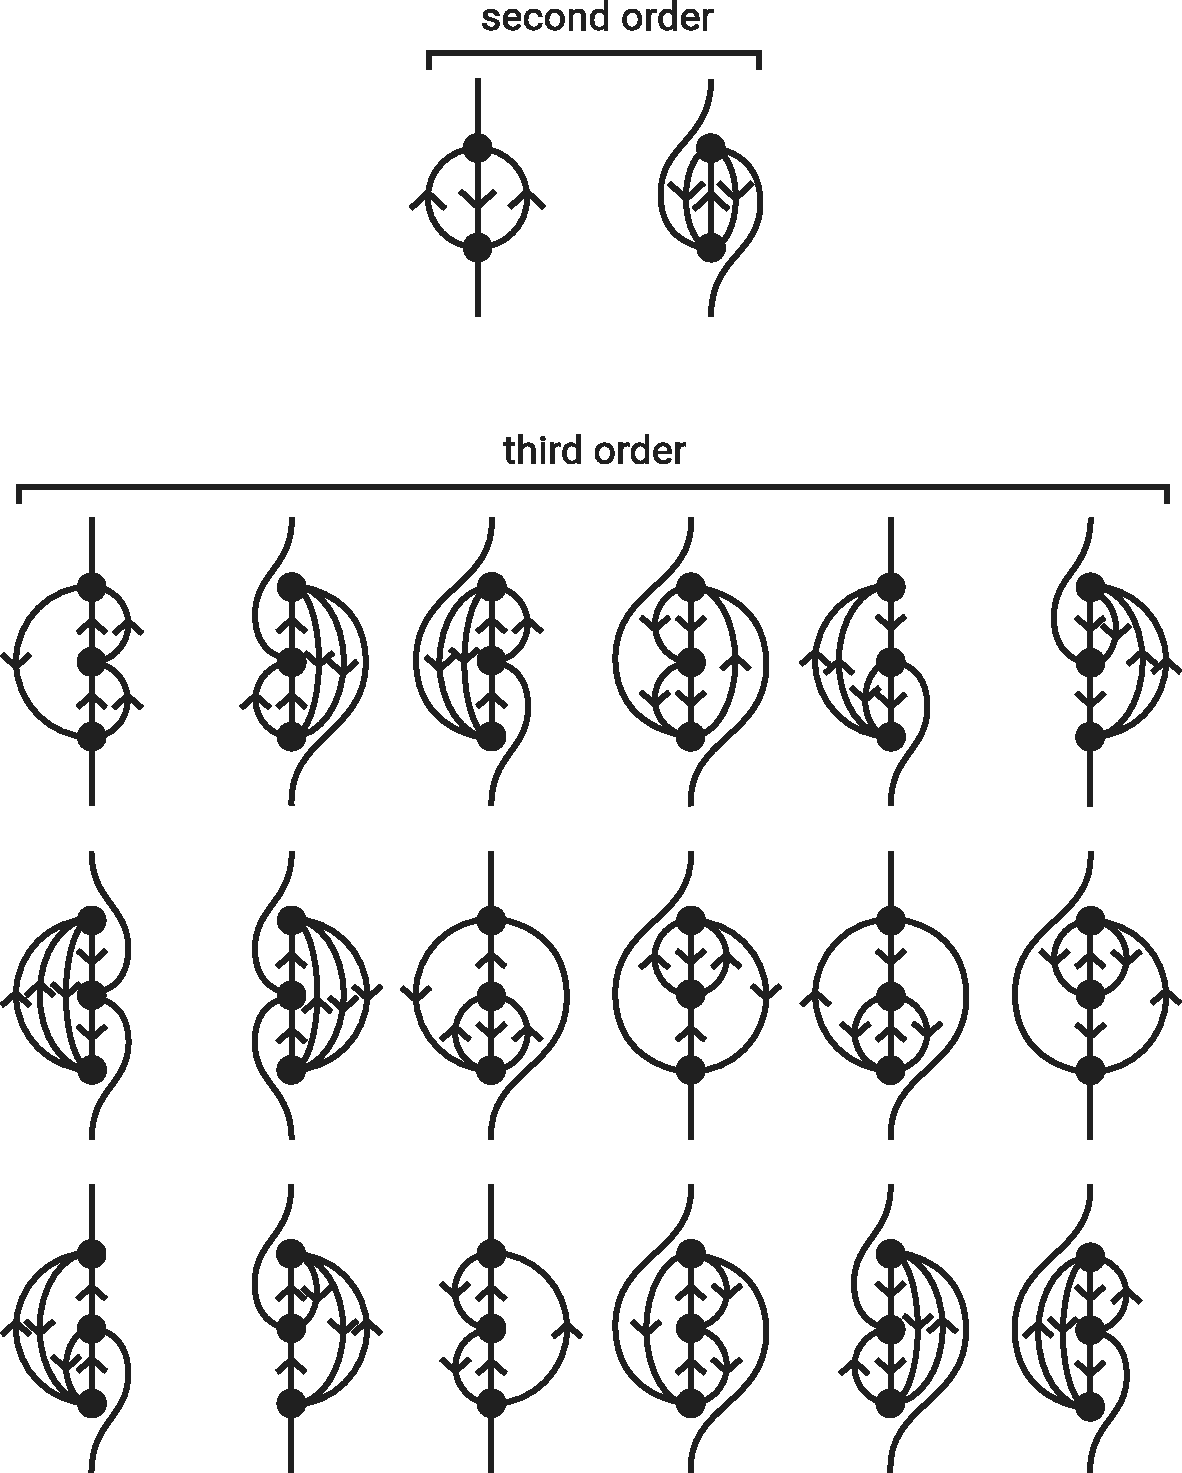
\includegraphics[width=.48\textwidth]{fig-diagrams-sfe}
\caption{Diagrammatic form of the second- and third-order QDPT corrections.  The diagrams are implicitly antisymmetrized (Hugenholtz diagrams), but also have implicit denominators as with many-body perturbation theory.}
\label{fig:diagrams-sfe}
\end{figure}

Since for this paper we are interested in the addition and removal energies, which involve one particle more or one particle less than a closed-shell state, we can take the label $u$ to be simply the label of the state that is added or removed from the closed-shell state $\Phi$.  With this realization, we can then express the perturbation expansion in terms of summations over matrix elements as we had done before for the IM-SRG flow equation, perhaps with the aid of Wick's theorem or diagrammatic techniques.  This leads to the following expression for the second-order correction:
\begin{gather*}
  \epsilon_p^{(2)} =
      \frac{1}{2} \sum_{i a b} \frac{n_i \bar{n}_a \bar{n}_b |V_{p i a b}|^2}{H^{[1]}_p + H^{[1]}_i - H^{[1]}_a - H^{[1]}_b}
    - \frac{1}{2} \sum_{i j a} \frac{n_i n_j \bar{n}_a |V_{i j p a}|^2}{H^{[1]}_i + H^{[1]}_j - H^{[1]}_p - H^{[1]}_a}
\end{gather*}
[[write out the full thing using $H^1_{p,p}$]]
The expression is depicted in Figure \ref{fig:diagrams-sfe}.  Since there are numerous terms in the third-order correction $\epsilon_p^{(3)}$, they are listed exclusively in a diagrammatic form in Figure \ref{fig:diagrams-sfe}.

Taking into account the perturbation corrections, one can obtain reasonably accurate addition and removal energies for single-particle states near the Fermi level via:
\begin{align*}
  \epsilon_p = H^{[1]}_{p, p} + \epsilon_p^{(2)} + \epsilon_p^{(3)}
\end{align*}

\subsection{Diffusion Monte Carlo}


Diffusion Monte Carlo (DMC) is a method for calculating the ground state
properties via a stochastic process akin to classical diffusion, refining an
approximate ground state density towards that of the exact ground state.  The
rules that govern the diffusion process are obtained by evolving the wave
function using what can be formally be thought of as the time-dependent
Schr\"odinger equation along imaginary time $\tau \equiv t / \mathrm{i}$:
\begin{align} \label{eq:itse}
  \frac{\partial}{\partial \tau} |\Phi(\tau)\rangle = \hat H |\Phi(\tau)\rangle
\end{align}
The solutions to this equation are not unlike the ordinary Schr\"odinger
equation with a slight but crucial difference in the exponent:
\begin{align*}
  |\Phi(\tau)\rangle = \mathrm e^{-\hat H \tau} |\Phi(0)\rangle
\end{align*}
where $|\Phi(0)\rangle$ is the initial wave function at $\tau = 0$ -- not to
be confused with the exact ground state of $\hat H$, which we denote
$|\Psi_0\rangle$ here.  If we decompose the wave function into a sum over the
eigenstates $|\Psi_n\rangle$,
\begin{align*}
  |\Psi(\tau)\rangle
  = \mathrm e^{-\hat H \tau} \sum_n c_n |\Psi_n\rangle
  = \sum_n c_n \mathrm e^{-E_n \tau} |\Psi_n\rangle
\end{align*}
we find that components of the wave function that have negative energy will
increase exponentially as $\tau \to \infty$, while those with positive energy
will decrease exponentially.  This property can be exploited to filter out the
undesirable components, leaving only the ground state energy.  To do this, we
require a trial energy $E_{\text{T}}$ -- a guess of the ground state energy --
and replace $\hat H$ in \eqref{eq:itse} with $(\hat H - E_{\text{T}})$ so
that, if our trial energy is good, all states but the ground states will
approximately vanish.

Diffusion Monte-Carlo (DMC) is a method used for refining a crude estimate to the ground state density into a better approximation to the exact ground state. The basic idea is to move multiple random walkers in position space with sampling rules which ensures convergence to a behavior representing a walk guided by the exact ground state density. Once a satisfying level of convergence is reached, expectation values are calculated by accumulating local estimates along the path of the walkers.

The equations representing the DMC algorithm is obtained by applying the projection operator $\hat{P}(\tau)$ on the crude trial state $\ket{\Psi_T}$
\begin{equation}
 \hat{P}(\tau)\ket{\Psi_T} \equiv \exp\left({-(\hat{H} - E_0)\tau}\right)\ket{\Psi_T}
\end{equation}
\noindent
where $\tau$ is a constant often described as imaginary time, and $E_0=\bra{\Psi_0}\hat{H}\ket{\Psi_0}$ is the ground state of the Hamiltonian $\hat{H}$. By expanding the trial state in the eigenfunctions of $\hat{H}$, the ground state is obtained up to a constant factor

\begin{equation}
 \label{eq:DMC_ExactProjection}
 \lim_{\tau\to\infty} \bra{\mathbf{r}}  \hat{P}(\tau) \ket{\Psi_T} = \braket{\Psi_0}{\Psi_T}\Psi_0(\mathbf{r}).
\end{equation}

Defining $\Phi(\mathbf{r}, \tau) \equiv \bra{\mathbf{r}}\hat{P}(\tau)\ket{\Psi_T}$, we obtain the state at a later time $\tau + \delta\tau$ through projection

\begin{align}
 \Phi(\mathbf{r}, \tau + \delta\tau) &= \bra{\mathbf{r}} P(\tau + \delta\tau) \ket{\Psi_T} \notag\\
 &= \bra{\mathbf{r}} \exp\left({-(\hat{H} - E_0)\delta\tau}\right) \hat{P}(\tau) \ket{\Psi_T} \notag\\
 &= \bra{\mathbf{r}} \exp\left({-(\hat{H} - E_0)\delta\tau}\right) \ket{\Phi(\tau)} \notag\\
 &= \int \D\mathbf{r}' \bra{\mathbf{r}} \exp\left({-(\hat{H} - E_0)\delta\tau}\right)\ket{\mathbf{r}'} \Phi(\mathbf{r}', \tau)\notag \\
 &\equiv \int \D\mathbf{r}' G(\mathbf{r}, \mathbf{r}'; \delta\tau) \Phi(\mathbf{r}', \tau). \label{eq:DMC_GreenFuncRevealed}
\end{align}

In practice, the ground state energy is a priori unknown, hence a trailing averaged value obtained from the converging DMC density is used. This energy is often referred to as the trial energy, and it is believed that with a sufficiently good trial state, the error due to this approximation is small.

The Green's function introduced in Eq.~(\ref{eq:DMC_GreenFuncRevealed}) has singularities due to the the Coulomb interaction term in $\hat{H}$. Due to Pauli exclusion these are not physical, nevertheless, in numerical implementations they are unpredictable and undesirable, hence we want to avoid them.

For evaluation of the local energy, the trial state is designed to cancel the Coulomb singularities by containing so-called correlation factors, however, this cancellation does not apply to the terms in the Green's function. In order to transfer this behavior to apply to the Green's function, a change to the formalism is introduced by iterating on a mixed density $f(\mathbf{r}, \tau) \equiv \Phi(\mathbf{r}, \tau)\Psi_T(\mathbf{r})$. Note that all previous arguments regarding convergence to the true ground state still applies for the new distribution.

Methods exist for transforming the mixed density into the pure density $|\Phi(\mathbf{r}, \tau)|^2$ \cite{abInitioMC}, but unless the pure density is explicitly needed (e.g.~for comparisons with other methods), this is strictly not necessary.

Additionally, to avoid issues regarding the positive definiteness of the mixed distribution, the nodes of the mixed density is fixed to those of the wave function of the trial state. This is known as the \textit{fixed node approximation} \cite{umrigar:2865, abInitioMC}. Again, given a sufficiently good trial state, the errors should be small.

The Green's function for the mixed density is given as \cite{umrigar:2865}

\begin{align}
  G(\mathbf{r}, \mathbf{r}'; \delta\tau)_f &= \bra{\mathbf{r}} \exp\left({\frac{1}{2}\nabla\cdot \left[\left(\nabla - \mathbf{F}(\mathbf{r})\right)\right] - \left(E_L(\mathbf{r}) - E_T\right)}\right)\ket{\mathbf{r}'} \label{eq:DMC_IS_GF_raw}\\
  &\propto e^{-\left[|\mathbf{r} - \mathbf{r}' - \frac{1}{2}\delta\tau\mathbf{F}(\mathbf{r})|^2/2\delta\tau\right]} \label{eq:DMC_IS_GF}\\
  &\qquad\times e^{-\left[\frac{1}{2}\left[E_L(\mathbf{r'}) + E_L(\mathbf{r})\right] - E_T\right]\delta\tau} + \mathcal{O}(\delta\tau^2), \notag
\end{align}
where
\begin{equation}
  \mathbf{F}(\mathbf{r}) = 2\Psi_T(\mathbf{r})^{-1} \nabla \Psi_T(\mathbf{r})
\end{equation}

\noindent
is the drift vector commonly referred to as the \textit{quantum force}.

The local energy
\begin{equation}
E_L(\mathbf{r}) = \Psi_T(\mathbf{r})^{-1}\hat{H} \Psi_T(\mathbf{r})
\end{equation}
is necessarily sampled from $|\Psi_T(\mathbf{r})|^2$ (ensured by using the Metropolis Algorithm \cite{abInitioMC}) to avoid undefined energies when sampling close to the nodes of $\Psi_T(\mathbf{r})$.

The Green's function from Eq.~(\ref{DMC_IS_GF_raw}) has been split into two for practical reasons; one part containing the kinetic terms, more specifically this represents a Fokker-Planck diffusion process, and a second part which is commonly referred to as a \textit{branching function}, which is an effective reweighing of a positions contribution to the overall density. Excluding branching we will simply sample from the density of the trial state.

In order dampen the errors introduced by splitting the Green's function, the time step $\delta\tau$ should be small. A value in the range of $10^{-3}$ to $10^{-4}$ is used in this work. High variance in energy samples requires a smaller time step to keep the branching controlled, since the fluctuations of the two are connected by Eq.~(\ref{eq:DMC_IS_GF}).

The name branching arise from the fact that in DMC, the weights are implemented as a probability of a given walker to copy or delete itself $n$ times, where $\langle n \rangle$ equals the branching term of Eq.~(\ref{eq:DMC_IS_GF}). Let $G_b$ denote the value of the branching function at a given position. Correct weighting is then ensured by guaranteeing $m = \max\left(\mathrm{floor}\left(G_b\right)-1, 0\right)$ branches with a probability $G_b - m$ of getting an additional branch. A branch is an identical copy of the corresponding walker, with an identical past but with a different future. When the number of requested branches is zero, the walker is removed from the simulation.


Initially, $N_w$ walkers are initialized to span $|\Psi_T(\mathbf{r})|^2$. This is ensured by using the Metropolis Algorithm. Moreover, importance sampling is ensured by sampling according to the kinetic term of  Eq.~(\ref{eq:DMC_IS_GF_raw}) \textit{cite solution langevin}

\begin{equation}
x_{i+1} = x_i + \frac{1}{2}\delta\tau F(\mathbf{r})_x + \xi,
\end{equation}
\noindent
where $\xi$ is a uniform distributed random number with variance $\mathrm{Var}(\xi) = 2D\delta\tau$. A typical value of $N_w$ in this work is 250 000.

For each time step, diffusion and branching repeats a given number of blocks $N_b$ for each walker. New branches are not active until the next time step, and if a walker hits zero branches the block repetition stops. During these block loops, the trial energy $E_T$ is sampled for use in the next time step $k+1$

\begin{equation}
 E_T^{k+1} = \frac{1}{M^{(k)}}\sum_{i=1}^{M^{(k)}} G_b(\mathbf{r}^{(k)}_i)E_L(\mathbf{r}^{(k)}_i),
\end{equation}
\noindent
where $M^{(k)}$ is the total number of samples obtained in cycle $k$. For this work we have found a value of $N_b = 100$ to be sufficient.

Several methods for estimating $E_0$ exist in the literature, one of which is simply an average of all $N_c$ trial energies calculated after $N_t$ thermalization cycles
\begin{equation}
 E_0 = \frac{1}{N_c-N_t}\sum\limits_{k=N_t}^{N_c} E_T^{(k)}.
\end{equation}
This is the relation we use in this work to obtain the DMC energies.

In this work, the trial state has been chosen to consist of a single Slater determinant (cite)
together with a single variational parameter Padé-Jastrow correlation function (cite).

The Slater determinant contains eigenstates $\phi_n(\mathbf{r})$ of Eq.~(\ref{eq:potential})
with a variational parameter $\alpha$ scaling the oscillator frequency $\omega$
such that $\omega\to\alpha\omega$ in all solutions:

\begin{equation}
 \phi_n(\mathbf{r}) = H_n(\sqrt{\alpha\omega}x)H_n(\sqrt{\alpha\omega}y)\exp(-\alpha\omega r^2),
\end{equation}

\noindent
where $H_n$ is the $n$'th level Hermite polynomial.


The eigenstates are selected such that the $N$ lowest lying energy eigenstates are selected (counting spin-degeneracy). Due to the Hamiltonian being spin independent we may split the Slater determinant into two equal parts -
one for each spin level (cite). The overall form of the trial state is as follows:

\begin{equation}
 \Psi_T(\mathbf{r}) = S(\mathbf{r}^\uparrow) S(\mathbf{r}^\downarrow) \prod_{i<j}^{N} J(r_{ij}),
\end{equation}

with

\begin{equation}
 S(\mathbf{r}^s) =  \left| \begin{array}{cccc}
\phi_1(\mathbf{r}^s_1) & \phi_2(\mathbf{r}^s_1)& \cdots & \phi_\frac{N}{2}(\mathbf{r}^s_1) \\
\phi_1(\mathbf{r}^s_2) & \phi_2(\mathbf{r}^s_2)& \cdots & \phi_\frac{N}{2}(\mathbf{r}^s_2) \\
\vdots & \vdots& \ddots & \vdots \\
\phi_1(\mathbf{r}^s_\frac{N}{2}) & \phi_2(\mathbf{r}^s_\frac{N}{2})& \cdots & \phi_\frac{N}{2}(\mathbf{r}^s_\frac{N}{2}) \\
 \end{array} \right|,
\end{equation}

and

\begin{equation}
 J(r_{ij}) = \exp\left(\frac{r_{ij}}{1 + \beta r_{ij}}\right),
\end{equation}

where $\mathbf{r}^s_i$ denotes $i$'th particle with spin $s$, and $r_{ij}$ is the relative distance between two electrons.
Since Metropolis Monte-Carlo only involves ratios of density functions, all normalization factors are skipped.

As a consequence of the variational principle, the optimal numeric values for $\alpha$ and $\beta$ can be found by minimizing the energy in the variational parameter space.
For this we have used the adaptive step gradient descent method (cite ASGD).

Using a single Slater determinant and a single variational parameter in the correlation function might at first glance seem insufficient,
however, the strength and robustness of DMC greatly succeeds at transforming this naive approximation into a very good estimate to the ground
state density. It should be mentioned that for systems where the single-particle Hamiltonian does not have analytical solutions, this approach
will indeed be insufficient due to low overlap between the initial and exact state.

A single Slater determinant and a simple correlation function opens up numerous optimization schemes which trivializes the CPU-time of most calculations.
We refer to Refs (cite optimization techniques) for more information.
Moreover, the most costly part of evaluating the single-particle eigenstates, the exponentials, is independent of the quantum number $n$, and can thus be tabulated once
for the entire calculation. This holds for the gradient and Laplacian needed in the quantum force and local energy, respectively, since the exponential shape is
preserved under differentiation.



\section{Results}
\label{sec:results}

\begin{figure}%[hbtp]
     \begin{center}
        \subfigure[Results for $N=6$ and $\omega=1.0$ ]{
            \label{fig:N6hw1}
            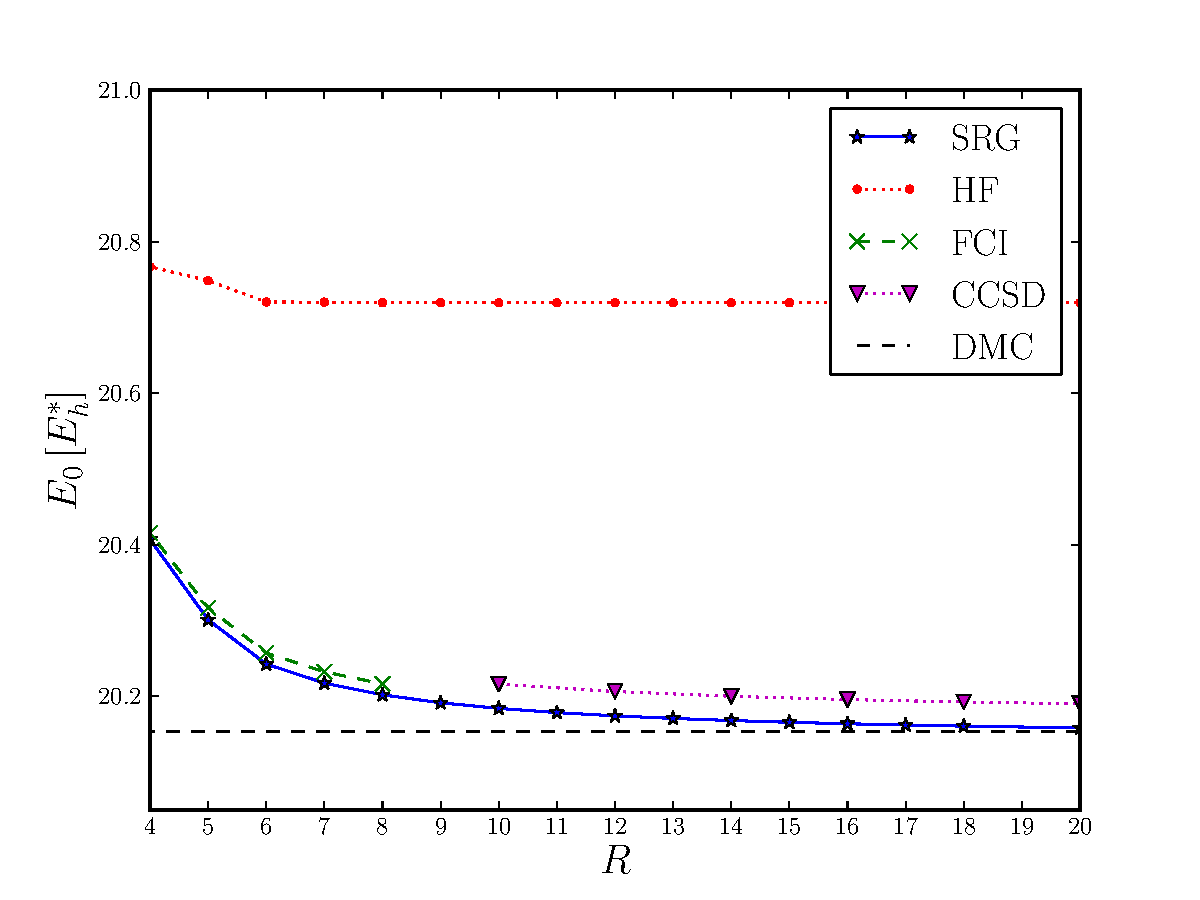
\includegraphics[width=0.38\textwidth]{figures/6parthw1.pdf}
        }
        \subfigure[Results for $N=6$ and $\omega=0.5$ ]{
           \label{fig:N6hw05}
           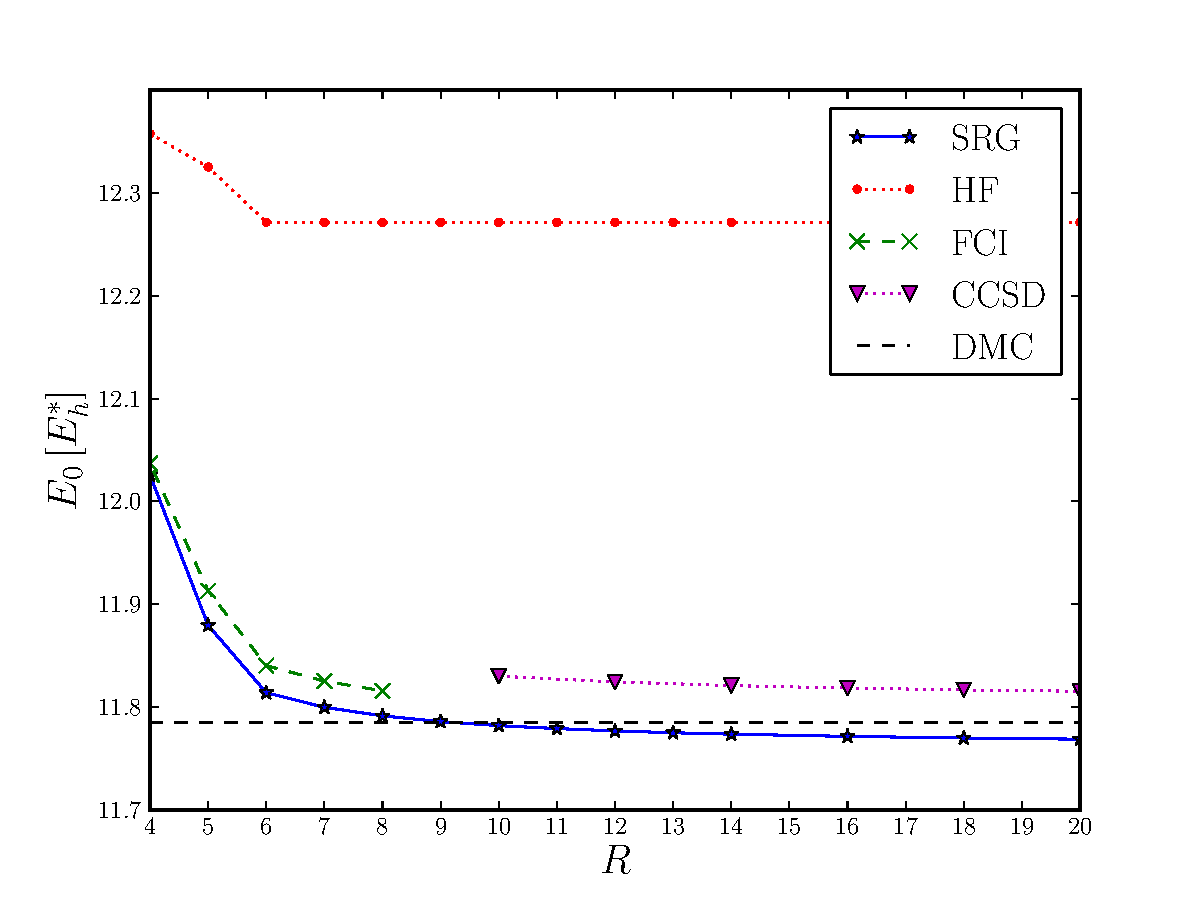
\includegraphics[width=0.38\textwidth]{figures/6parthw05.pdf}
        }\\ %  ------- End of the first row ----------------------%
        \subfigure[Results for $N=6$ and $\omega=0.28$ ]{
            \label{fig:N6hw028}
            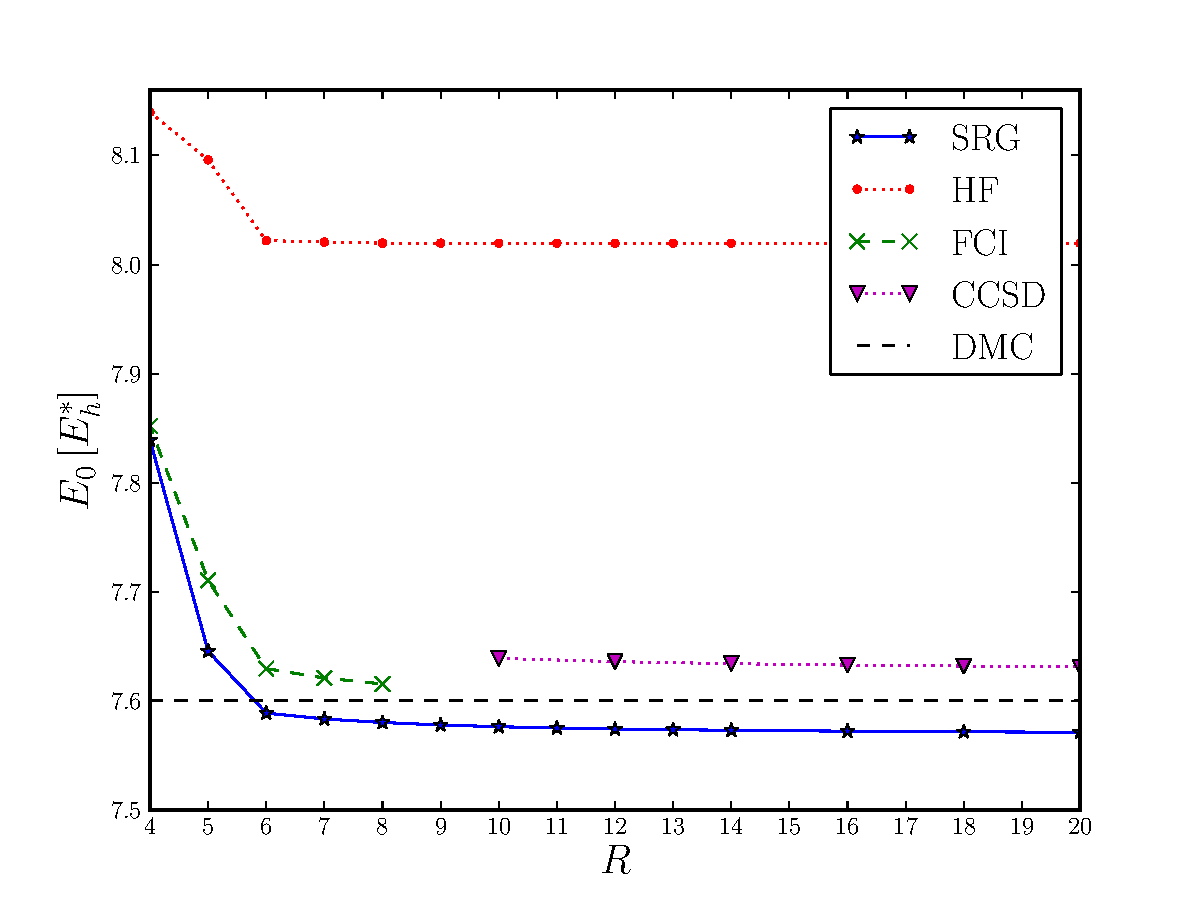
\includegraphics[width=0.38\textwidth]{figures/6parthw028.pdf}
        }
        \subfigure[Results for $N=6$ and $\omega=0.1$ ]{
            \label{fig:N6hw01}
            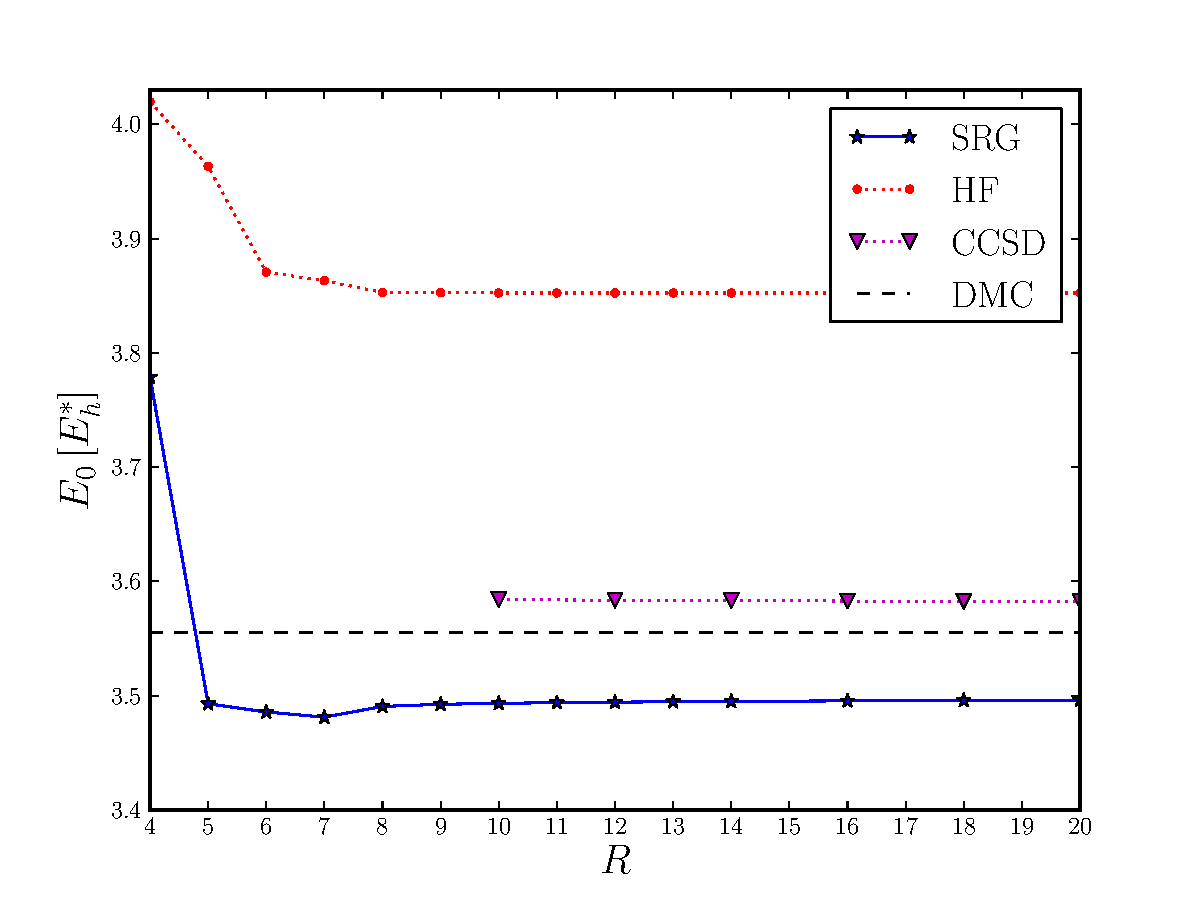
\includegraphics[width=0.38\textwidth]{figures/6parthw01.pdf}
        }
    \end{center}
    \caption{Comparison of our IM-SRG(2) ground state energies (SRG)
      for circular quantum dots for $N=6$ and $\omega=1.0$
       The results are compared with diffusion Monte Carlo (DMC),
      coupled cluster at the level of singles and doubles (CCSD), full
      configuration interaction (FCI) and Hartree-Fock calculations
      (HF) as functions of the number of major oscillator shells
      $R$. A harmonic oscilaltor basis has been used, with an
      unrenormalized Coulomb repulsion and White's generator. All
      energies in atomic units.}
   \label{fig:N6}
\end{figure}





\begin{figure}%[hbtp]
     \begin{center}
        \subfigure[Results for $N=12$ and $\omega=1.0$ ]{
            \label{fig:N12hw1}
            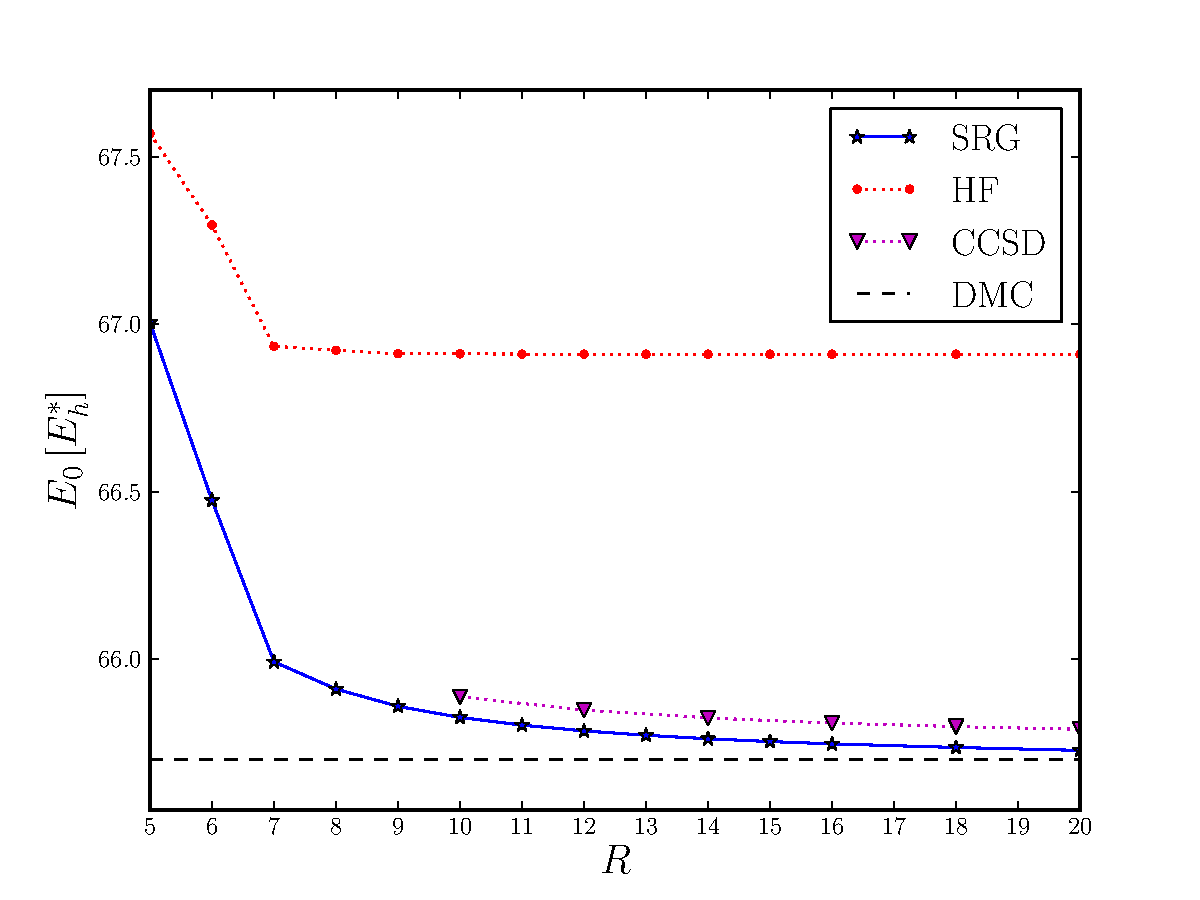
\includegraphics[width=0.38\textwidth]{figures/12parthw1.pdf}
        }
        \subfigure[Results for $N=12$ and $\omega=0.5$ ]{
           \label{fig:N12hw05}
           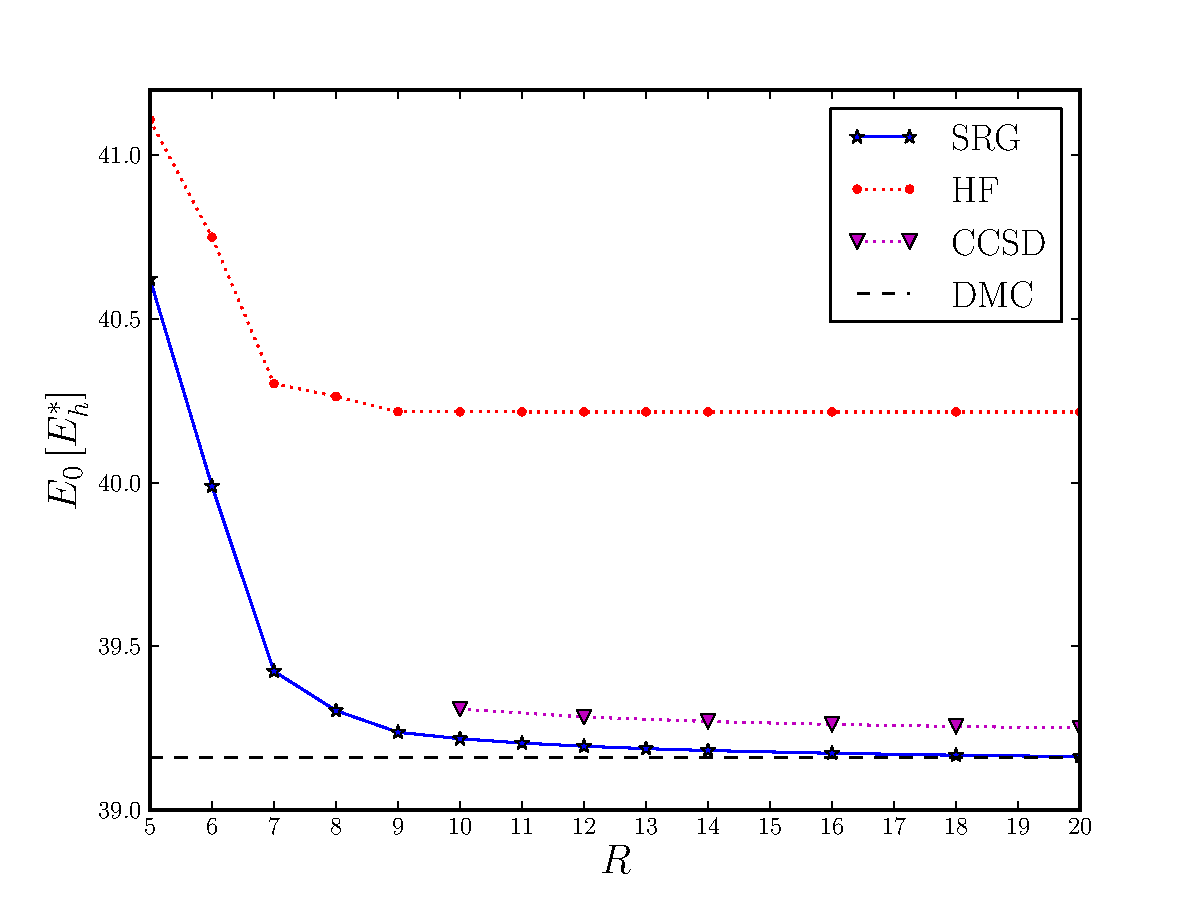
\includegraphics[width=0.38\textwidth]{figures/12parthw05.pdf}
        }\\ %  ------- End of the first row ----------------------%
        \subfigure[Results for $N=12$ and $\omega=0.28$ ]{
            \label{fig:N12hw028}
            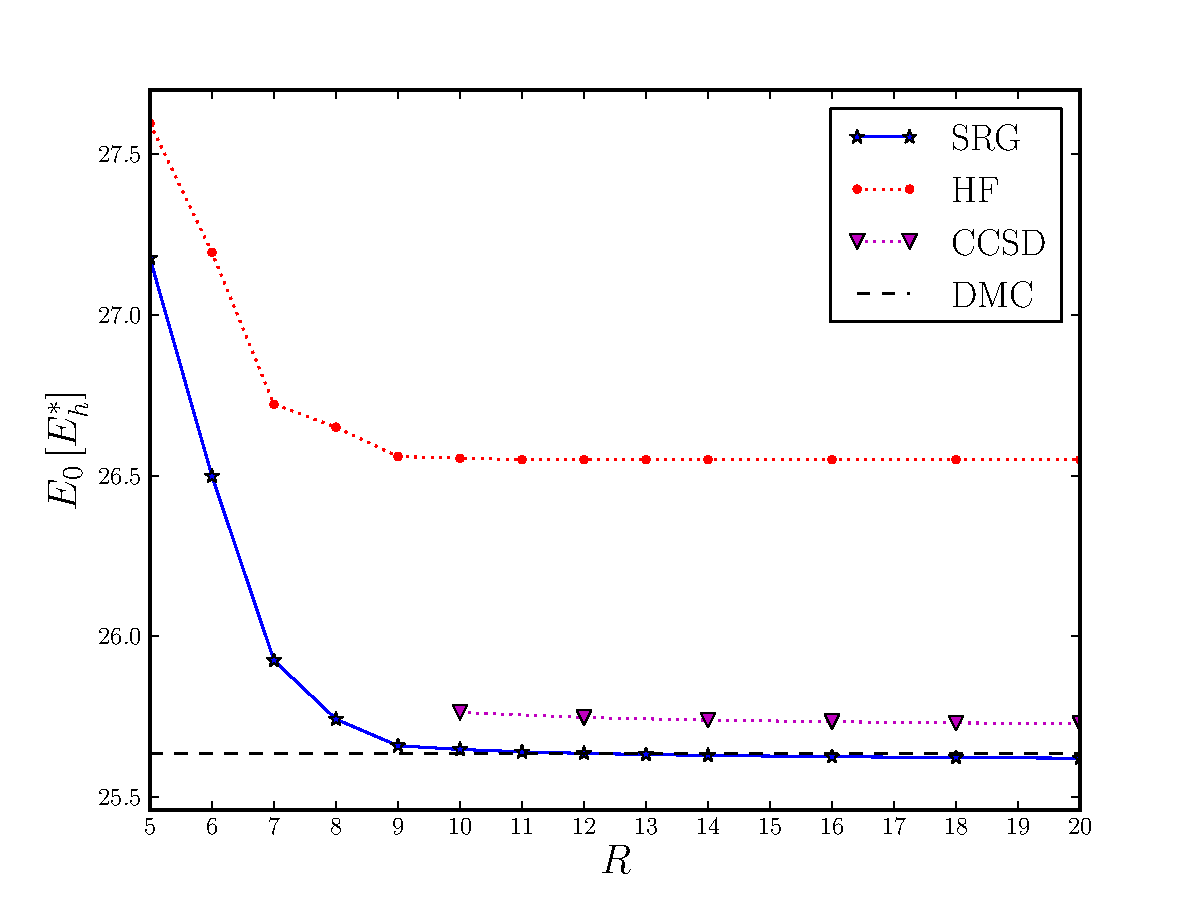
\includegraphics[width=0.38\textwidth]{figures/12parthw028.pdf}
        }
        \subfigure[Results for $N=12$ and $\omega=0.1$ ]{
            \label{fig:N12hw01}
            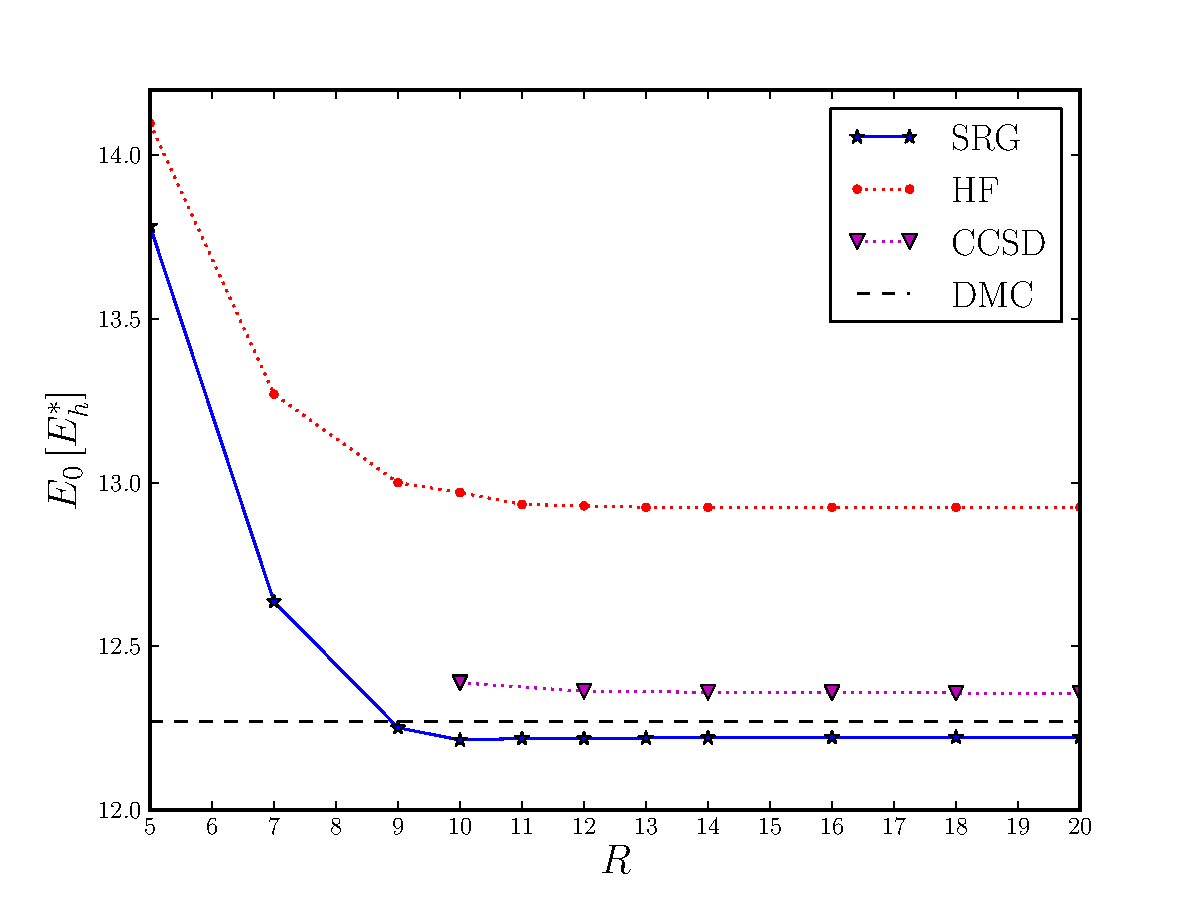
\includegraphics[width=0.38\textwidth]{figures/12parthw01.pdf}
        }
    \end{center}
    \caption{Comparison of our IM-SRG(2) ground state energies (SRG)
      for circular quantum dots for $N=12$ and different values of
      $\omega$. The results are compared with diffusion Monte
      Carlo (DMC), coupled cluster at the level of singles and doubles
      (CCSD), full configuration interaction (FCI) and Hartree-Fock
      calculations (HF) as functions of the number of major oscillator
      shells $R$. A harmonic oscilaltor basis has been used, with an
      unrenormalized Coulomb repulsion and White's generator. All
      energies in atomic units.}
   \label{fig:N12}
\end{figure}





\begin{figure}%[hbtp]
     \begin{center}
        \subfigure[Results for $N=20$ and $\omega=1.0$ ]{
            \label{fig:N20hw1}
            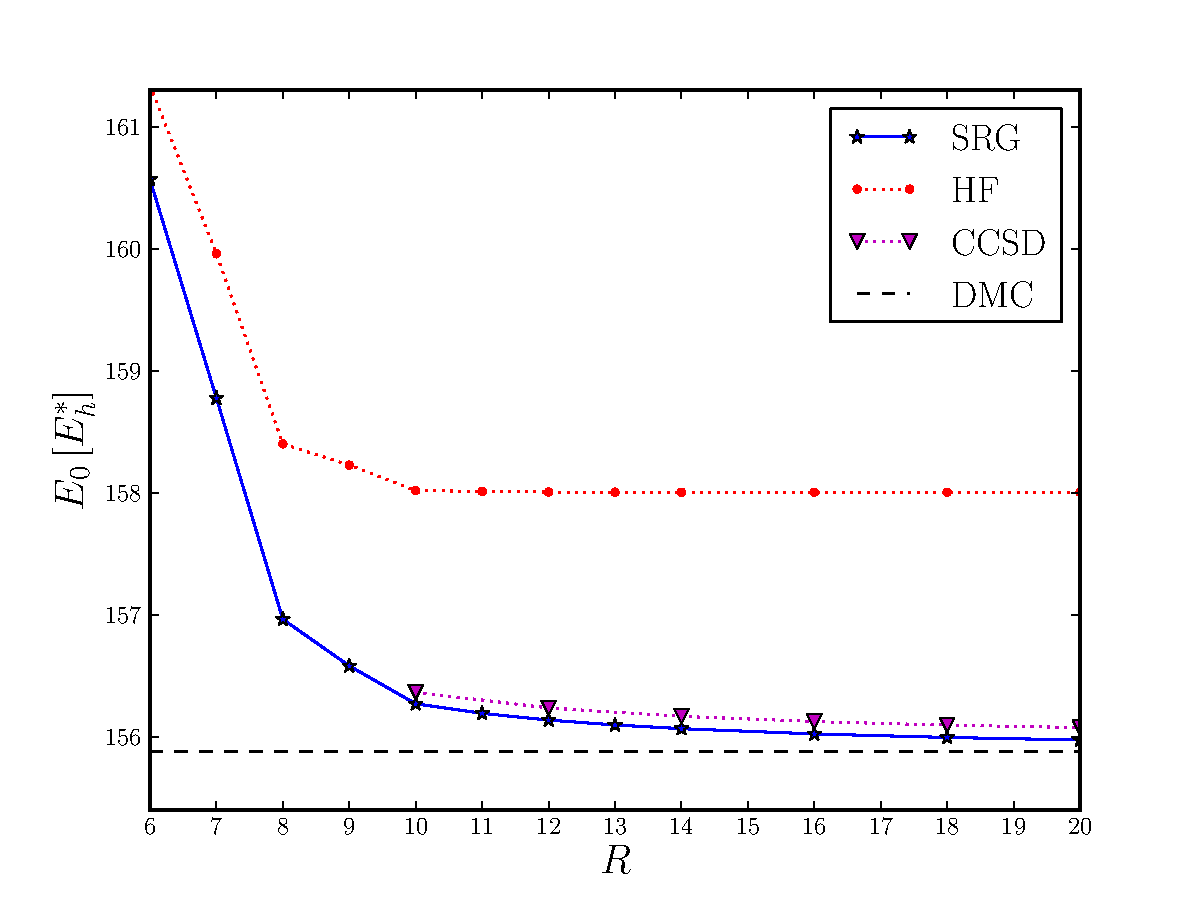
\includegraphics[width=0.38\textwidth]{figures/20parthw1.pdf}
        } \subfigure[Results for $N=20$ and $\omega=0.5$ ]{
           \label{fig:N20hw05}
           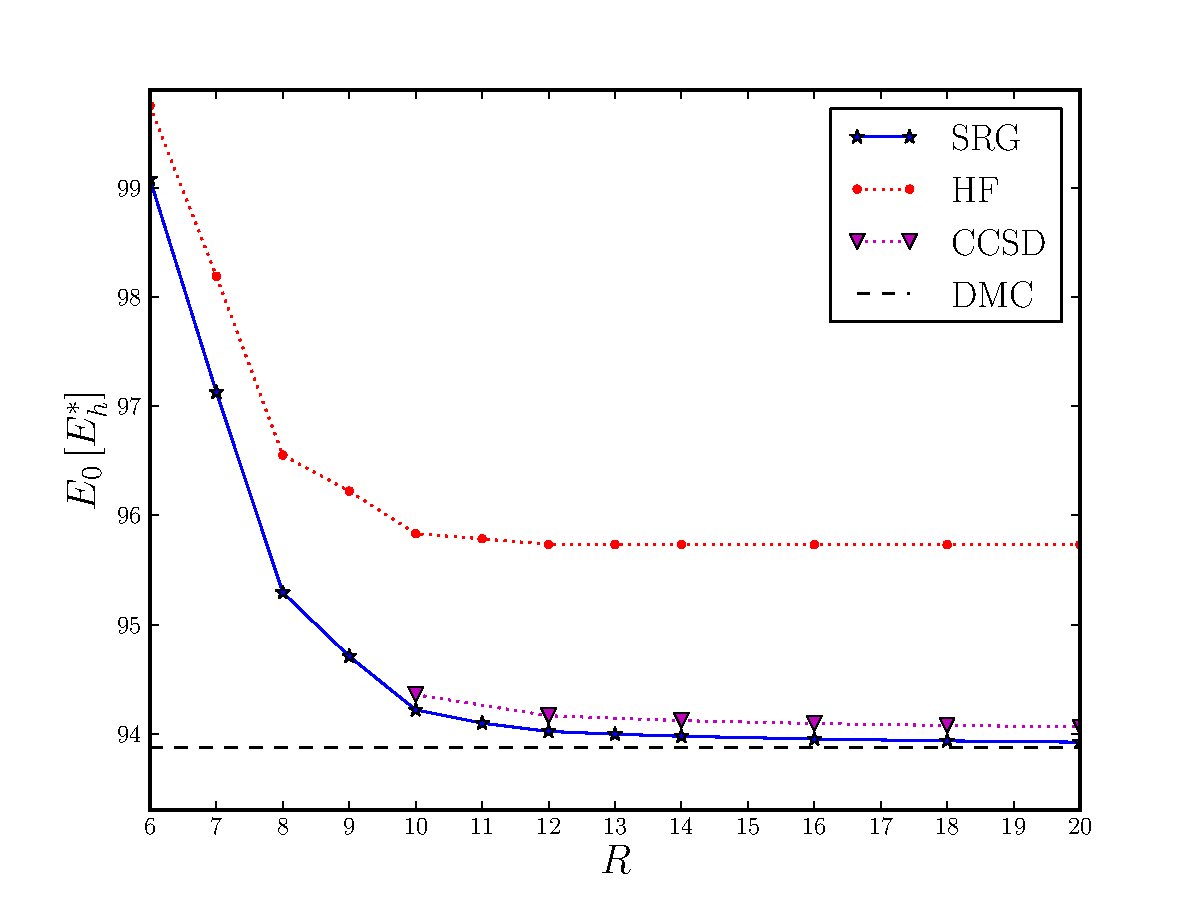
\includegraphics[width=0.38\textwidth]{figures/20parthw05.pdf}
        }\\ % ------- End of the first row ----------------------%
        \subfigure[Results for $N=20$ and $\omega=0.28$ ]{
            \label{fig:N20hw028}
            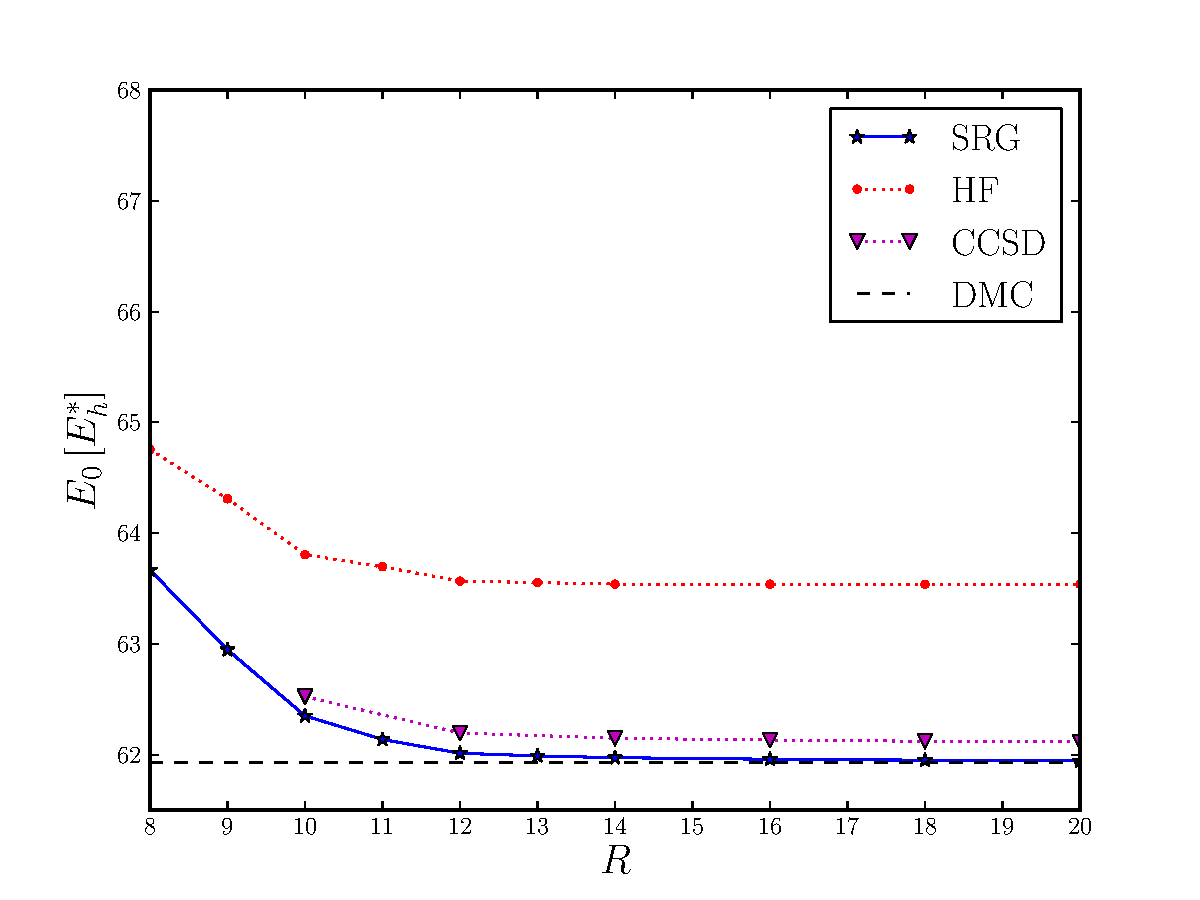
\includegraphics[width=0.38\textwidth]{figures/20parthw028.pdf}
        } \subfigure[Results for $N=20$ and $\omega=0.1$ ]{
            \label{fig:N20hw01}
            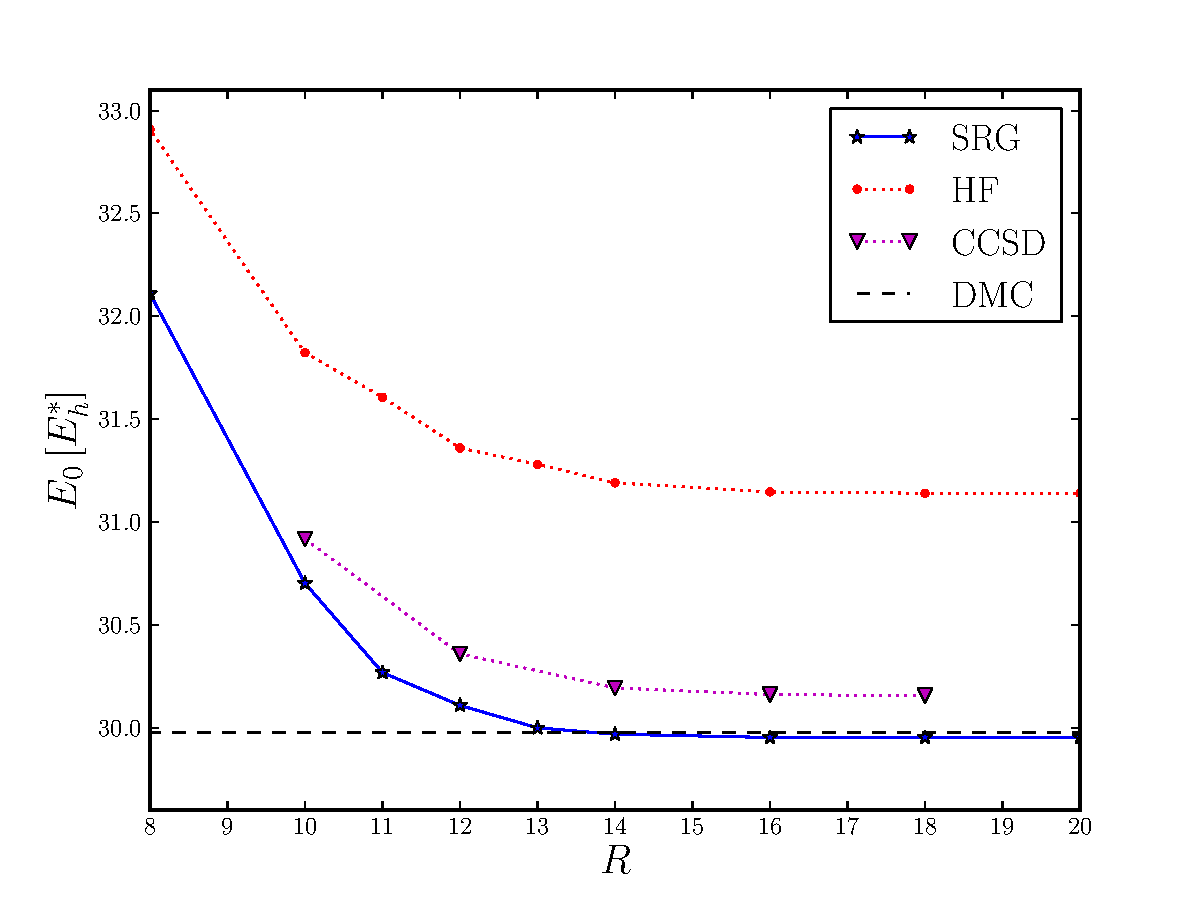
\includegraphics[width=0.38\textwidth]{figures/20parthw01.pdf}
        }
    \end{center}
    \caption{Comparison of our IM-SRG(2) ground state energies (SRG)
      for circular quantum dots for $N=20$ and different values of
      $\omega$. The results are compared with diffusion Monte
      Carlo (DMC), coupled cluster at the level of singles and doubles
      (CCSD), full configuration interaction (FCI) and Hartree-Fock
      calculations (HF) as functions of the number of major oscillator
      shells $R$. A harmonic oscilaltor basis has been used, with an
      unrenormalized Coulomb repulsion and White's generator. All
      energies in atomic units.}
   \label{fig:N20}
\end{figure}



\begin{figure}%[hbtp]
     \begin{center}
        \subfigure[Results for $N=30$ and $\omega=1.0$ ]{
            \label{fig:N30hw1}
            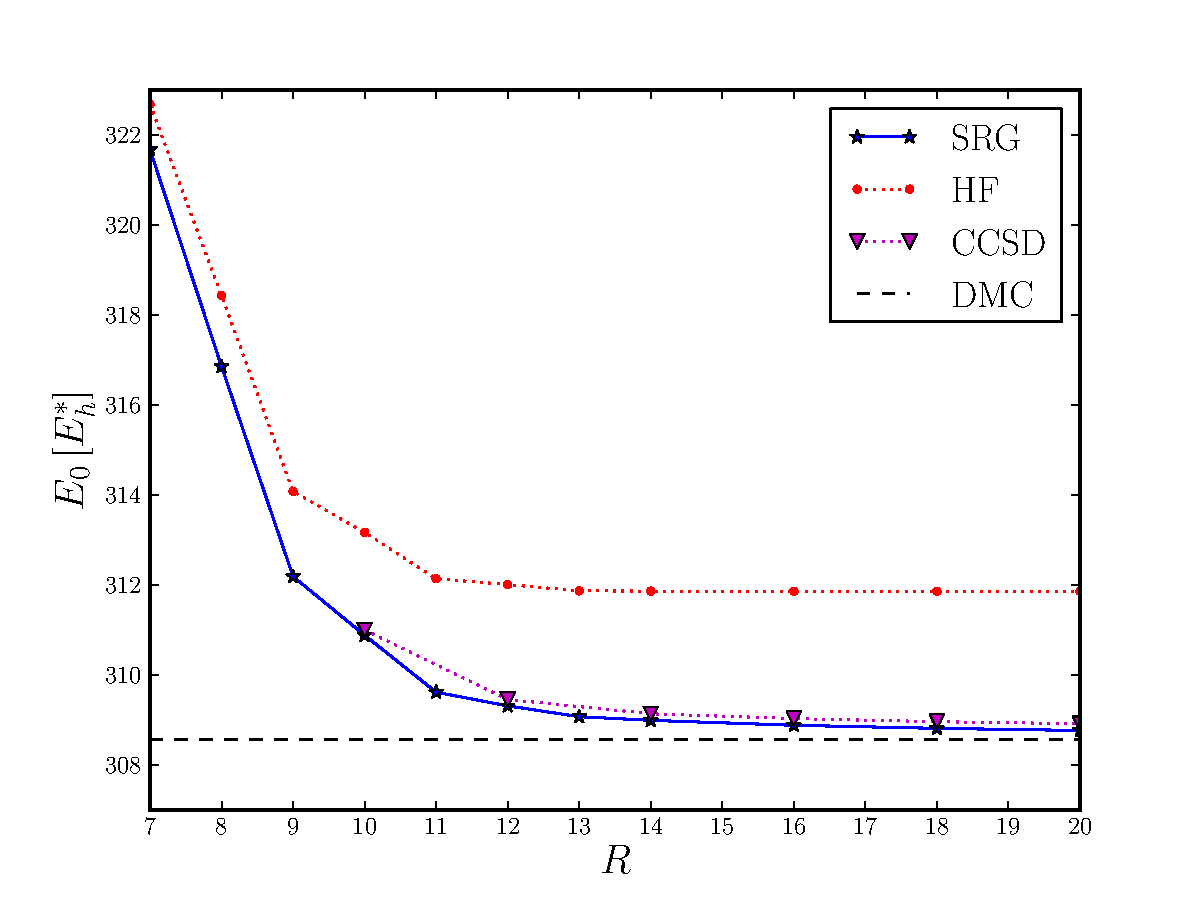
\includegraphics[width=0.38\textwidth]{figures/30parthw1.pdf}
        } \subfigure[Results for $N=30$ and $\omega=0.5$ ]{
           \label{fig:N30hw05}
           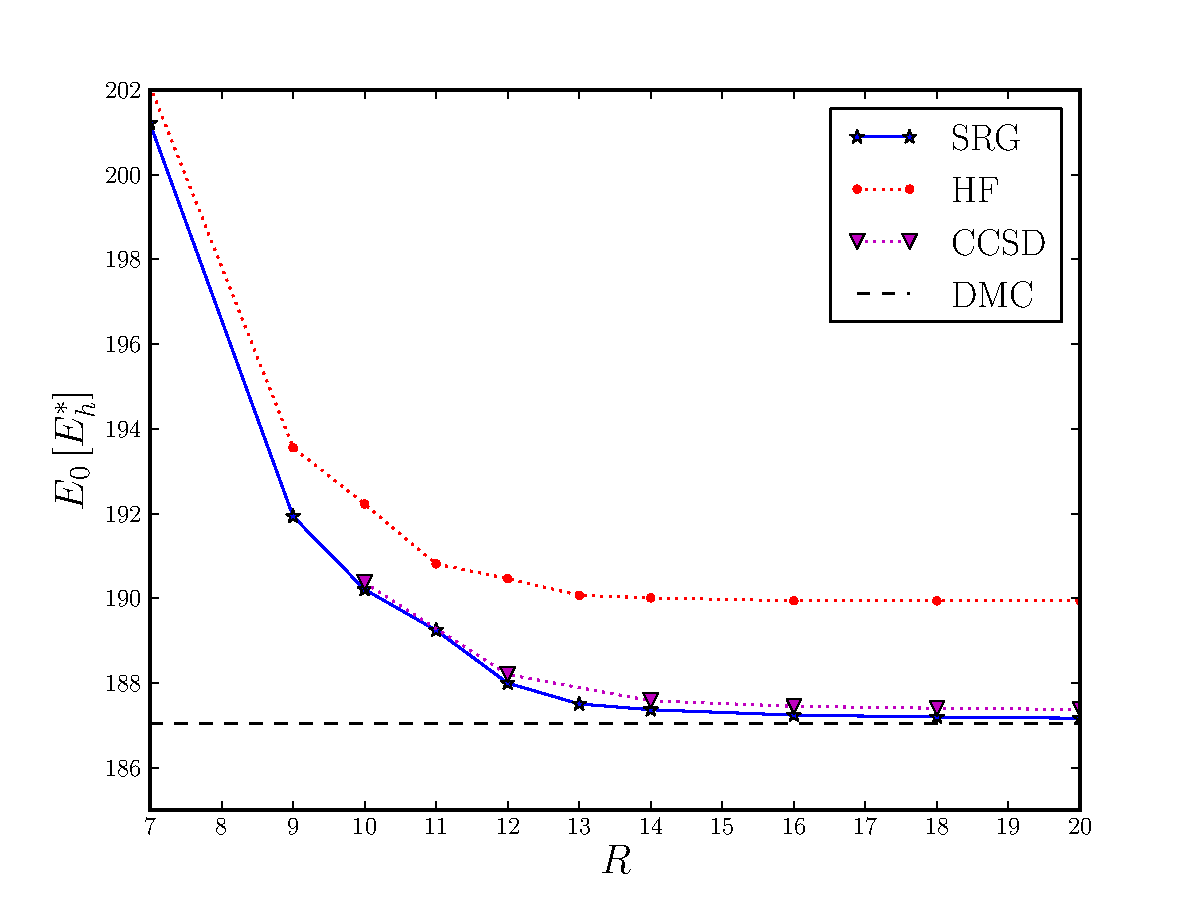
\includegraphics[width=0.38\textwidth]{figures/30parthw05.pdf}
        }\\ % ------- End of the first row ----------------------%
        \subfigure[Results for $N=30$ and $\omega=0.28$ ]{
            \label{fig:N30hw028}
            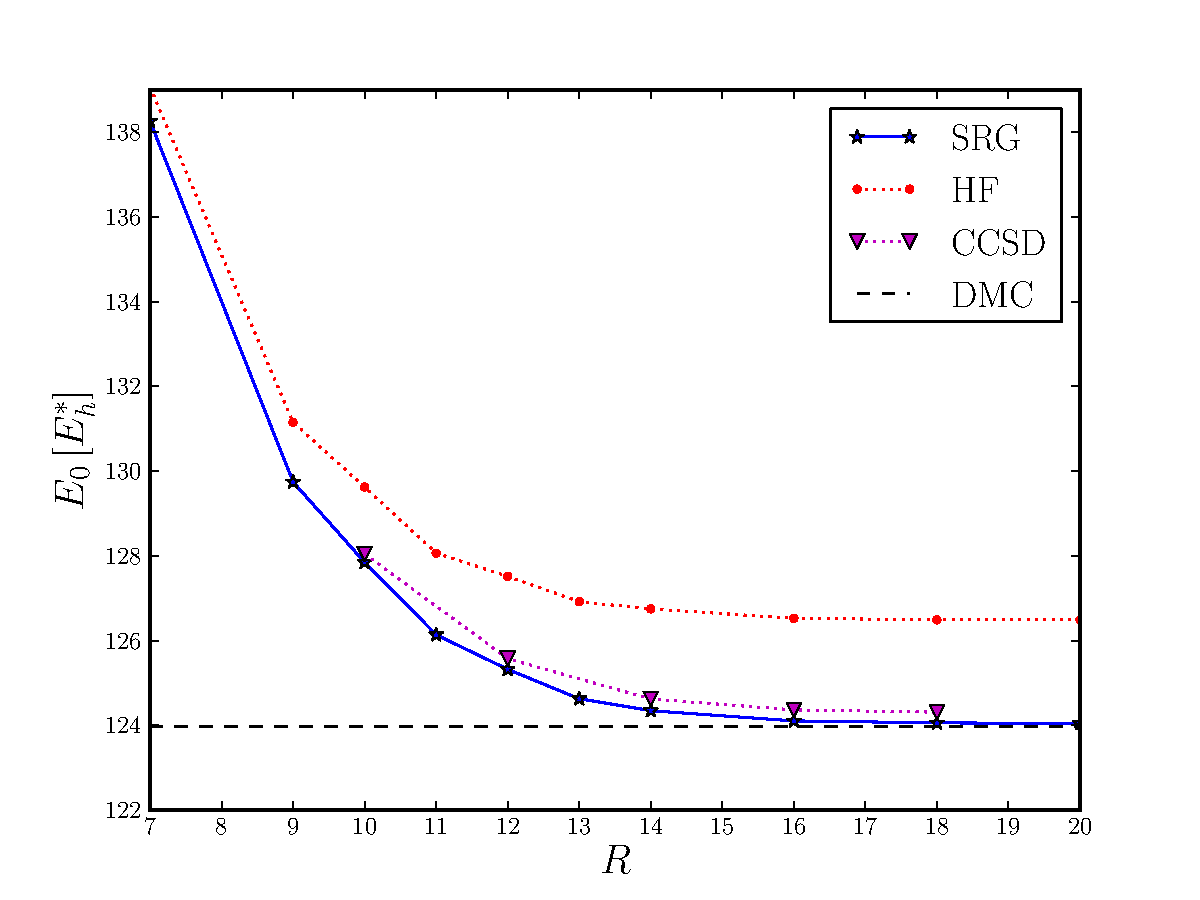
\includegraphics[width=0.38\textwidth]{figures/30parthw028.pdf}
        } \subfigure[Results for $N=30$ and $\omega=0.1$ ]{
            \label{fig:N30hw01}
            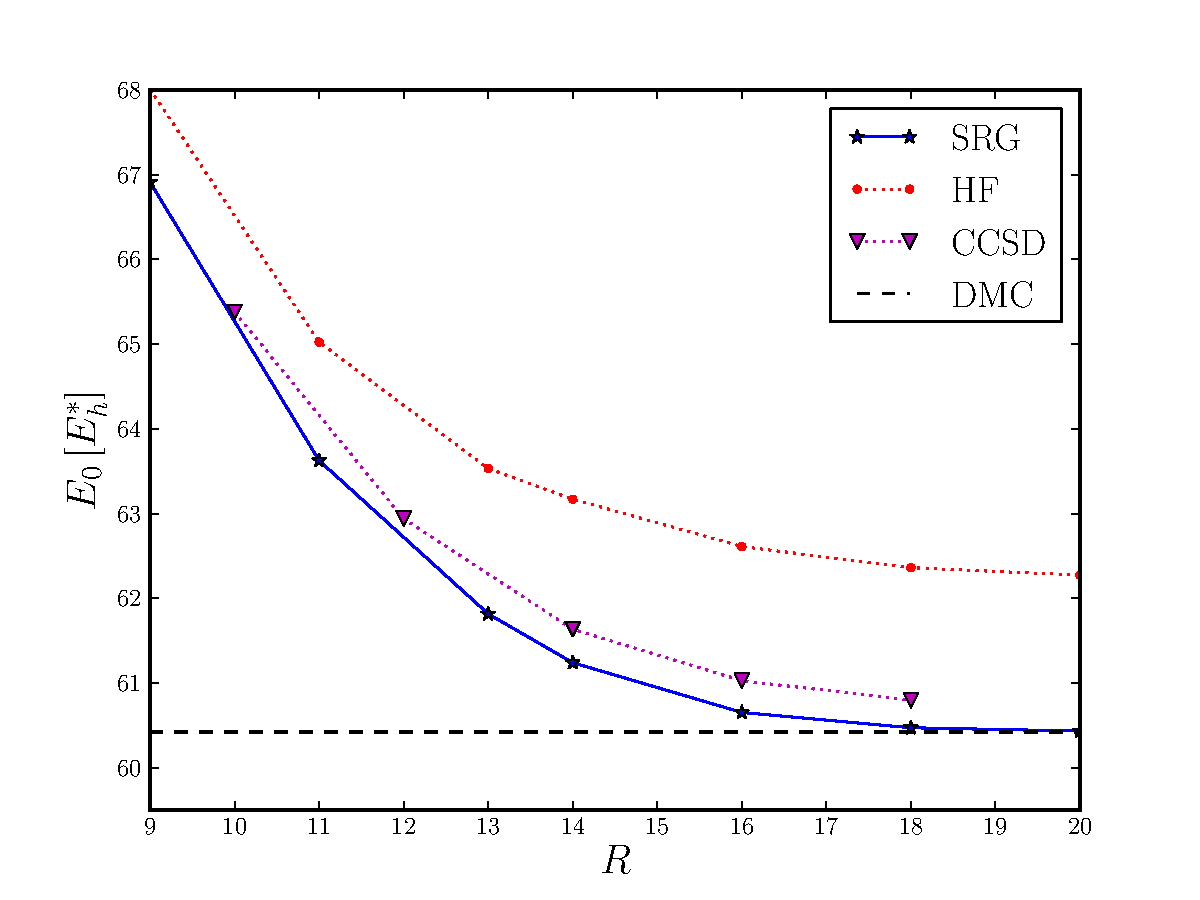
\includegraphics[width=0.38\textwidth]{figures/30parthw01.pdf}
        }
    \end{center}
    \caption{Comparison of our IM-SRG(2) ground state energies (SRG)
      for circular quantum dots for $N=30$ and different values of
      $\omega$. The results are compared with diffusion Monte
      Carlo (DMC), coupled cluster at the level of singles and doubles
      (CCSD), full configuration interaction (FCI) and Hartree-Fock
      calculations (HF) as functions of the number of major oscillator
      shells $R$. A harmonic oscilaltor basis has been used, with an
      unrenormalized Coulomb repulsion and White's generator. All
      energies in atomic units.}
   \label{fig:N30}
\end{figure}



\begin{figure}%[hbtp]
     \begin{center}
        \subfigure[Results for $N=42$ and $\omega=1.0$ ]{
            \label{fig:N42hw1}
            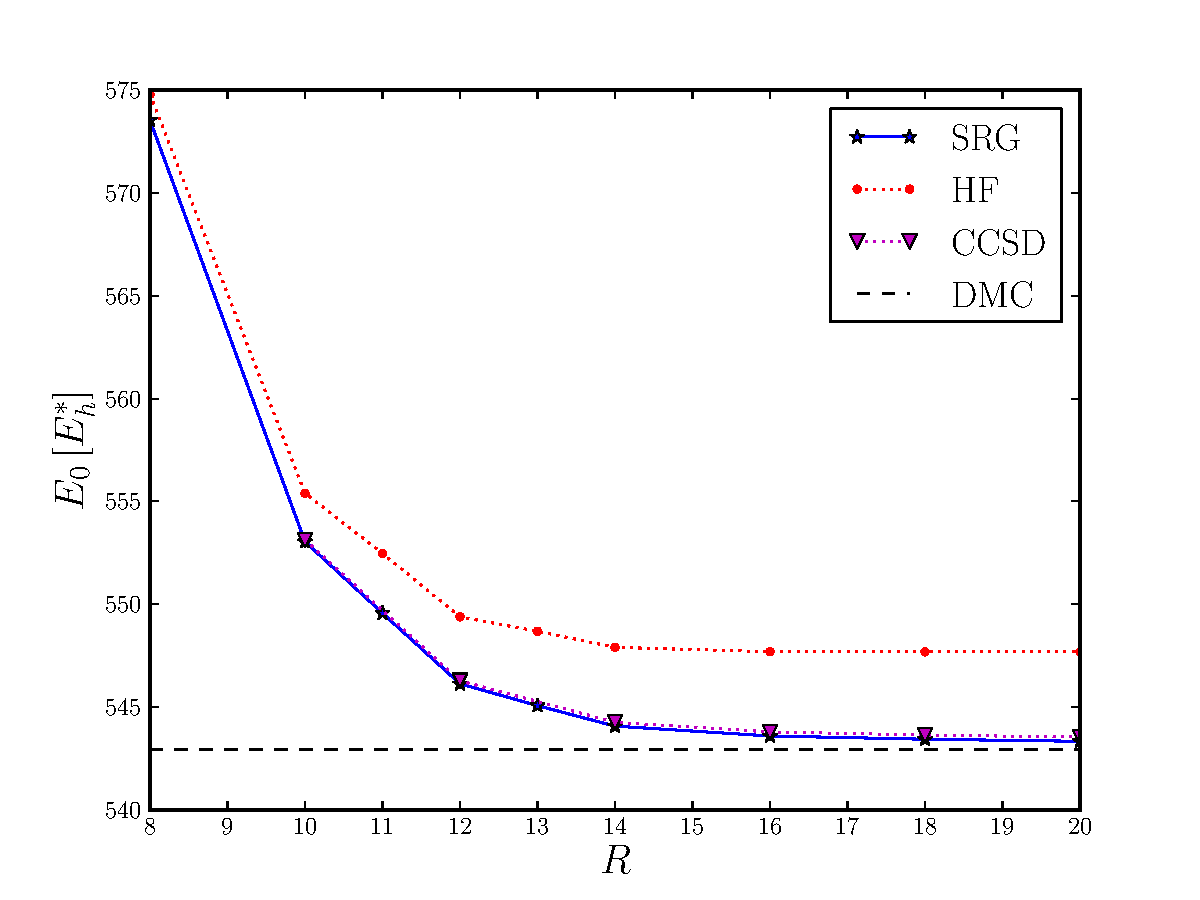
\includegraphics[width=0.38\textwidth]{figures/42parthw1.pdf}
        } \subfigure[Results for $N=42$ and $\omega=0.5$ ]{
           \label{fig:N42hw05}
           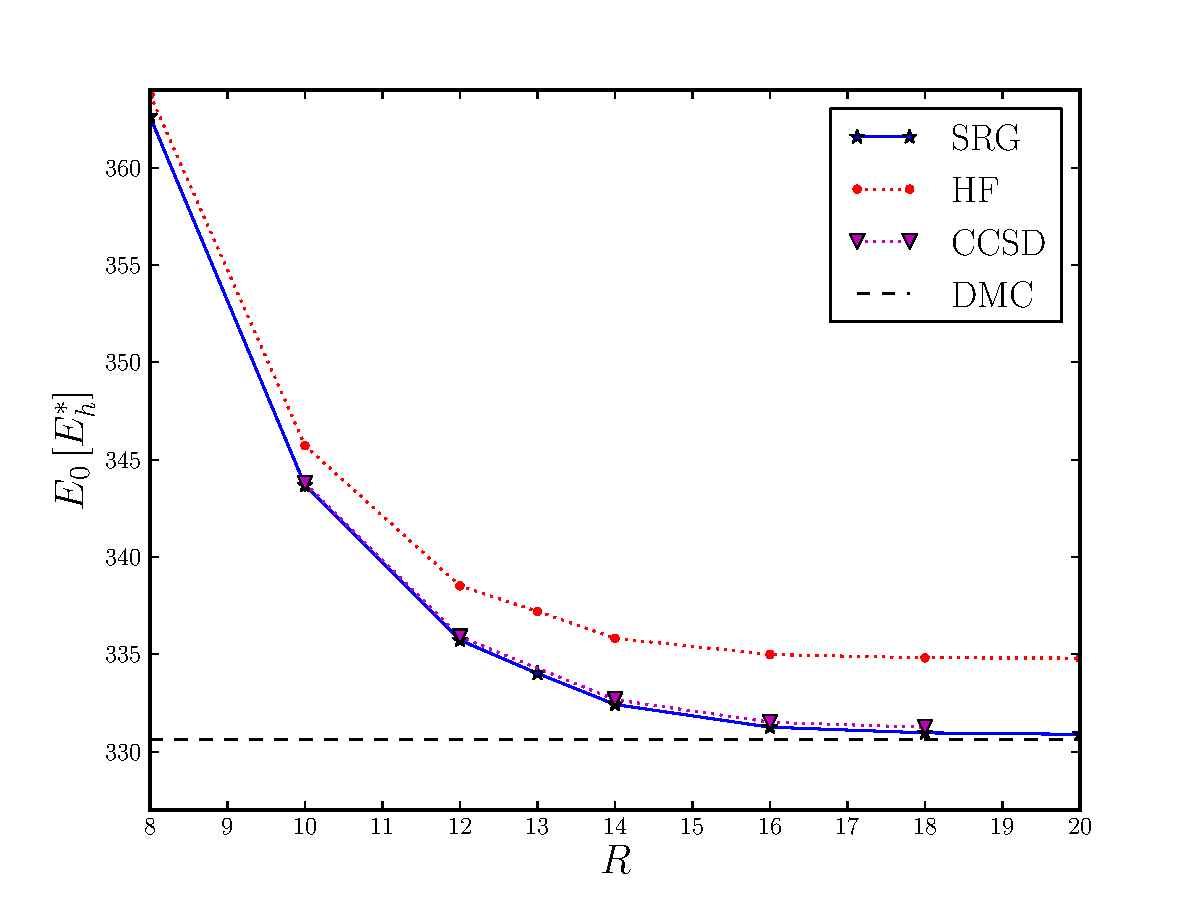
\includegraphics[width=0.38\textwidth]{figures/42parthw05.pdf}
        }\\ % ------- End of the first row ----------------------%
        \subfigure[Results for $N=42$ and $\omega=0.28$ ]{
            \label{fig:N42hw028}
            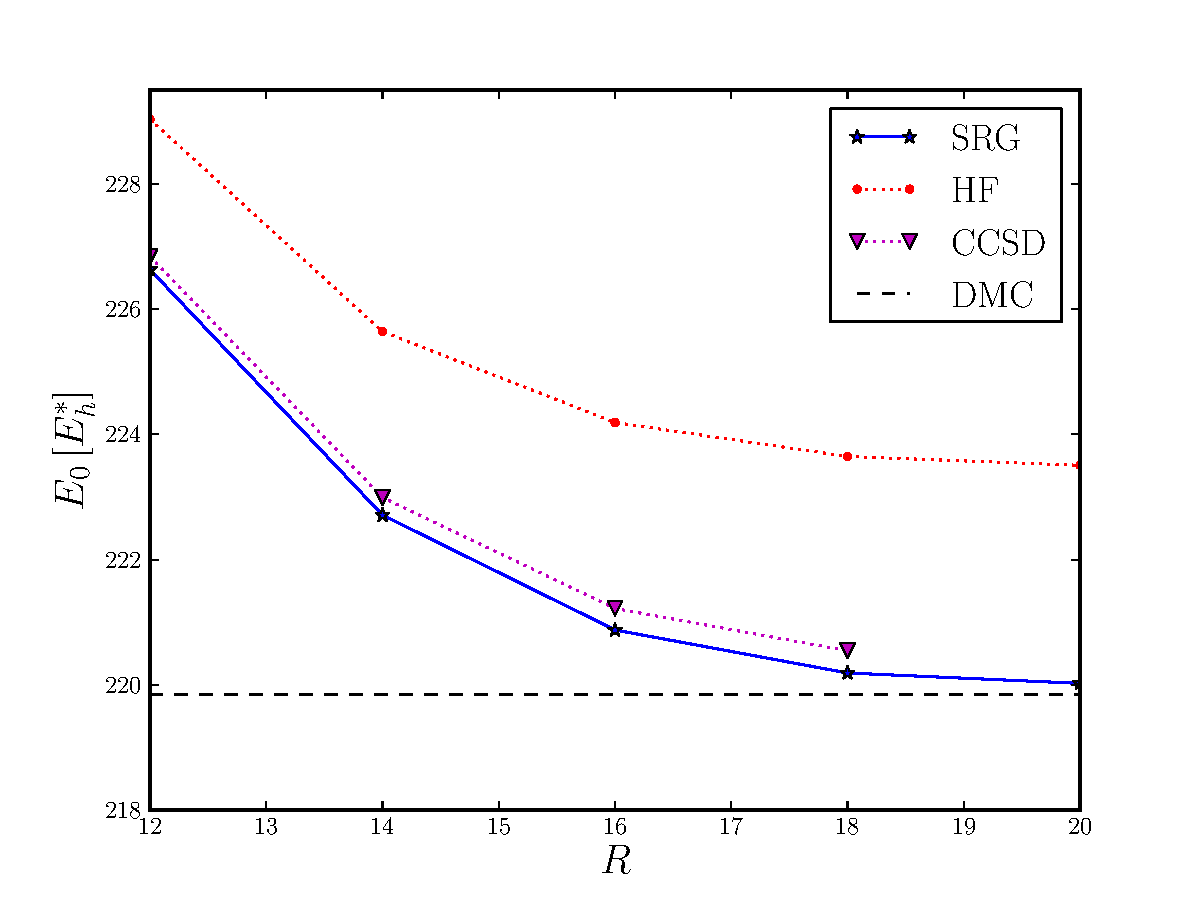
\includegraphics[width=0.38\textwidth]{figures/42parthw028.pdf}
        } \subfigure[Results for $N=42$ and $\omega=0.1$ ]{
            \label{fig:N42hw01}
            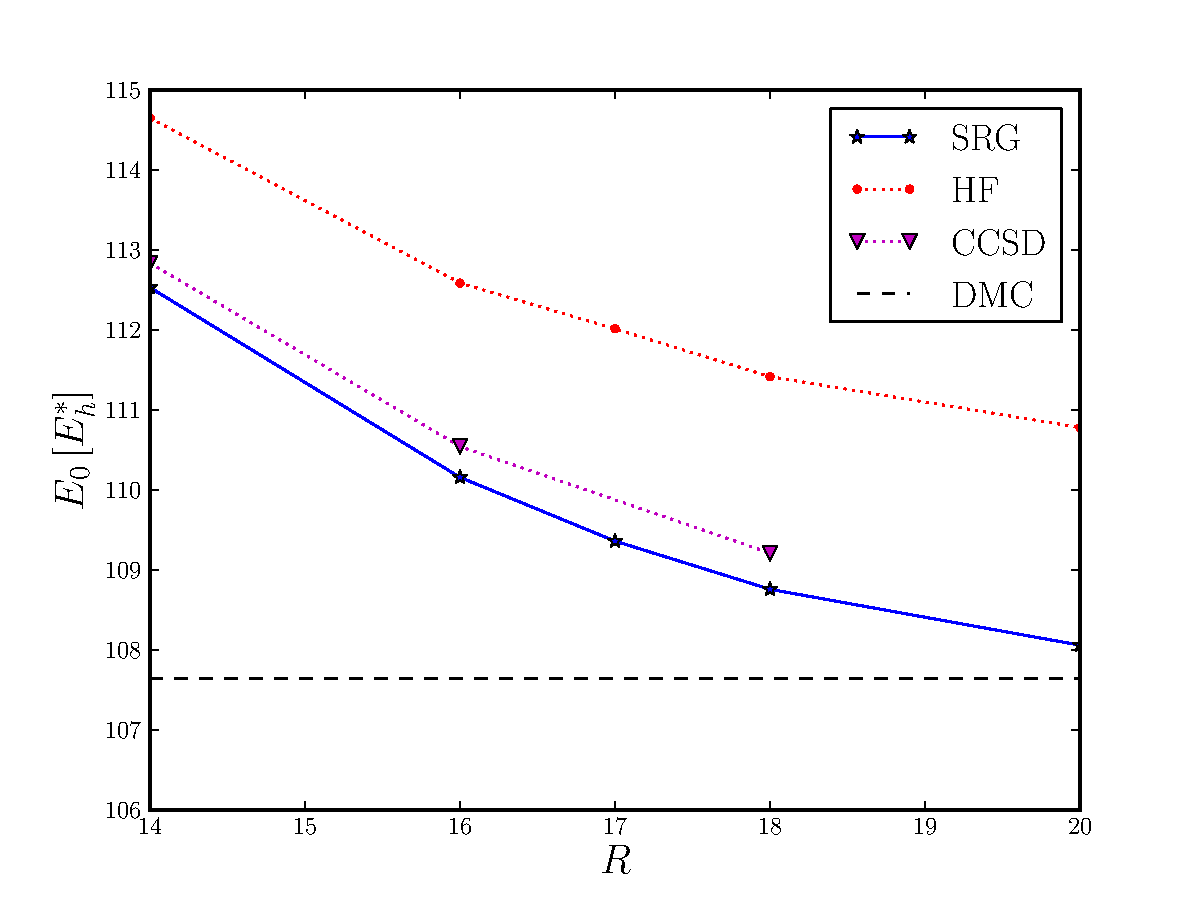
\includegraphics[width=0.38\textwidth]{figures/42parthw01.pdf}
        }
    \end{center}
    \caption{Comparison of our IM-SRG(2) ground state energies (SRG)
      for circular quantum dots for $N=42$ and different values of
      $\omega$. The results are compared with diffusion Monte
      Carlo (DMC), coupled cluster at the level of singles and doubles
      (CCSD), full configuration interaction (FCI) and Hartree-Fock
      calculations (HF) as functions of the number of major oscillator
      shells $R$. A harmonic oscilaltor basis has been used, with an
      unrenormalized Coulomb repulsion and White's generator. All
      energies in atomic units.}
   \label{fig:N42}
\end{figure}



\begin{table}
\begin{center}
\caption{Ground state energy (in atomic units) of a circular quantum
  dot, with $N$ particles and oscillator frequency $\omega$. The
  IM-SRG(2) results are given for $R=20$ shells (except for the $N=56$
  results which are for $R=18$), employing a Hartree-Fock basis, a
  bare Coulomb interaction and White's generator. For $N=42$ and
  $\omega=0.1$ results are presented up to $R=22$ major shells. The
  results labelled IM-SRG(2)$_{R\rightarrow \infty}$ are obtained
  using the extrapolation formula of Eq.().}
\label{tab:SRGDMC-R20}
\begin{tabular}{ccccc}
\hline\hline
$N$ & $\omega$ & IM-SRG(2) &IM-SRG(2)$_{R\rightarrow \infty}$ & DMC \\
\hline
6 & 1.0 & 20.1583 & 20.1468   & 20.1593(1) \\
& 0.5&11.7690  & 11.7631 &11.7848(1) \\
& 0.28& 7.5713 &   7.5695 &7.6002(1) \\
& 0.1& 3.4962  &  3.4977 &3.5539(1)\\
\hline
12&1.0 & 65.7280 & 65.6990  & 65.7001(1) \\
&0.5 &39.1631 &  39.1473 & 39.1596(1)\\
&  0.28&25.6212 &  25.6140& 25.6358(1)\\
&  0.1&12.2223 &  12.2234 & 12.2698(1)\\
\hline
20& 1.0&155.9737 & 155.9130  & 155.8822(1)\\
&  0.5&93.9219 &   93.8853 &93.8752(1)\\
&  0.28&61.94362 & 61.9240 &61.9268(1) \\
&  0.1&29.95263 &29.9565  & 29.9779(1)\\
\hline
30& 1.0& 308.7673 & 308.6053 & 308.5627(2) \\
 & 0.5& 187.1671& 186.8340 &187.0426(2)\\
 & 0.28&124.0410 & 123.7171 & 123.9683(2) \\
 & 0.1& 60.4319& 60.1158 & 60.4205(2)\\
\hline
42& 1.0&543.3398 & 543.3304 & 542.9428(8) \\
 & 0.5&330.8885 & 330.8425 & 330.6306(2)\\
 & 0.28&220.0226 & 219.9534y &219.8426(2) \\
 & 0.1& 107.7851&  106.8074& 107.6389(2)\\
 \hline
56& 1.0& 880.4159 &  & 879.3986(6) \\
 & 0.5& 538.8199 & & 537.353(2)\\
 & 0.28&360.83689  &  & 358.145(2) \\
\hline
\end{tabular}
\end{center}
\end{table}




In Figure \ref{fig:gs} we show the calculated ground state energies from
Hartree-Fock, second-order (M\o ller-Plesset) perturbation theory (MPPT), and
IMSRG.  The exact result from diffusion Monte Carlo (DMC) is also shown as a
dashed line in systems where it is known \cite{PhysRevB.84.115302}.

Both perturbation theory and IMSRG add corrections in addition to the
Hartree-Fock results to recover the correlation energy and they do quite well
in recovering the correlation energy in the system.  Compared with MPPT, IMSRG
generally converges faster, although does not always converge to the DMC
result.  Generally speaking, IMSRG is closer to the DMC result as the number
of particles increases.

There are a few cases where the IMSRG over-corrects the result, leading to a
ground state energy that is lower than the exact result.  This is not
unexpected given that, unlike Hartree-Fock, IMSRG is non-variational.  These
tend to occur when the number of particles is few, or the frequency is very
low (high correlation).  However, MPPT does not do much better in the high
frequency regimes as it often converges slower than IMSRG.

[[Q: should we discuss the absolute/relative correction plots?]]

For our addition and removal energy calculations, the results are summarized
in Figure \ref{fig:add} and Figure \ref{fig:rm} respectively.  The figures
show the the addition/removal energies for Hartree-Fock, combined with IM-SRG
and/or QDPT (Hartree-Fock is always included, as usual) [[better way to
explain this? the figure labels are somewhat misleading too]].  The DMC
results are also shown via dashed lines where they are known.

From these results, we see that the QDPT corrections add a substantial
contribution to the results of both Hartree-Fock with and without IM-SRG.
[[quantify ``substantial'' numerically]]

For the IM-SRG results, there is a small asymmetry between the behavior of our
removal and addition energies: we find that removal energies tend to be more
accurate and its behavior is relatively stable with respect to the number of
shells. [[why]]

Interestingly, the addition energy of Hartree-Fock with second-order QDPT
appears to surpass the accuracy of that of IM-SRG with second-order QDPT.
This is likely coincidental, as the third-order QDPT dramatically worsens the
result.

Both Hartree-Fock and IM-SRG results worsen as the frequency decreases, which
is not unexpected since the correlations become much more dominant.  The
Hartree-Fock appears to perform much worse, however, as the results converge
much more slowly as the number of shells increases.

We also note that IM-SRG with 2 particles and frequency 0.1 generally fail to
give any result as the ODE solver eventually leads to divergence [[Why?]]
This seems to be a particular quirk associated with this specific system and
does not usually occur in other systems except in a few extreme, isolated
cases where there are far too few unoccupied states.

\section{Conclusions}
\label{sec:conclusions}

We demonstrated the use various many-body theories, Hartree-Fock method, M\o
eller-Plesset perturbation theory, IM-SRG, as well as quasidegenerate
perturbation theory to calculate ground state as well as addition and removal
energies of two-dimensional quantum dots.  We showed that these methods, when
combined, can give a good approximate description of the systems at moderate
cost compared to near-exact but much more expensive methods such as FCI and
DMC.

For ground state energy, we showed that the convergence of IM-SRG is generally
faster than that of MPPT, and the results are typically closer to the exact
results.  Similarly, we found that IM-SRG improves the rate of convergence of
the addition and removal energies, both as the order of perturbation theory
increases and as the number of shells increases.

There are several directions in which the calculations may be improved.  One
can attempt to improve the IM-SRG approximation by incorporating some of the
missing higher-body terms in the commutator.  This would also provide some
insight into the rate of convergence with respect to the operator truncation.
While some of the higher-body terms can be rather costly to compute --
rendering a full 3-body IM-SRG quite expensive -- certain additional
approximations may be made to alleviate this without incurring the full cost
of evolving 3-body operators [[Ref?]].

[[As noted earlier [[haven't written that yet]], the application of IM-SRG
removes a large portion of the QDPT diagrams, which is beneficial as it
increases the efficiency of the QDPT calculations.  However, many of these
diagrams can also be eliminated further through an infinite resummation scheme
[[Any good refs for this?]], which would further reduce the number of diagrams
in QDPT, especially those of lower order, whic would likely increase the
accuracy of the result.]]

It would also be useful to investigate how the results obtained with finite
number of shells in the basis are related to those obtained with an infinite
number of shells in the basis.  [[Ref: paper on IR/UV extrapolation]] With a
good theoretical foundation, a model of how the observables converge with
respect to the size of the basis may be used to extrapolate the results to
infinite-basis limit.  This would also enable us to perform cheaper
calculations with fewer shells and optimistically extrapolate results for
large systems that would be otherwise infeasible to compute.

We note that this calculation was done entirely using the traditional approach
of using a high-order ODE solver to solve the flow equation.  A new technique
developed by T. Morris [[Ref?]] uses an alternative approach that obviates the
need for a high-order ODE solver, leading to much more efficient computations
and also allowing operators of other observables to be evolved with greater
ease.  Implementing this approach would be beneficial as it would allows us to
study the accuracy and convergence of other observables beyond energy and
energy differences.

Implementation-wise, our current code constructs the two-particle basis as
simple Slater determinants without any angular momentum coupling.  This
approach is often referred to as \textit{m-scheme} in nuclear physics.  This
method is simple and works well for general systems, but it does not fully
exploit the circular symmetry present in the quantum dot system.  A more
efficient approach is to use angular momentum coupling to generate the
two-particle basis, which is known as \textit{j-scheme} in nuclear physics.
Combined with the symmetries of the Hamiltonian, this can significantly reduce
the amount of computation required in this system, albeit at the cost of
increasing the complexity of the implementation.

A more technical issue is its lack of parallelization: currently, the code
makes very little use of parallelism and therefore does not scale well on
modern clusters.  As the problem is not embarrassingly parallel, implementing
parallelism does introduce additional complications that must be considered.
Distributing the workload across multiple nodes can significantly reduce the
cost of the calculations, allowing larger systems to be studied.

\begin{acknowledgments}
 This work was supported by the
National Science Foundation Grant No.~PHY-1404159
(Michigan State University) and by the Research
Council of Norway under contract ISP-Fysikk/216699.
\end{acknowledgments}

\bibliography{paper}
\bibliographystyle{apsrev4-1}
\end{document}



\documentclass[aps,twocolumn,showpacs,floatfix,nofootinbib,preprintnumbers,superscriptaddress,amsmath,amssymb]{revtex4-1}

\usepackage{graphicx}
\usepackage{epsfig}
\usepackage{bm}
\usepackage{color}
\usepackage{float}
\usepackage{dcolumn}
\usepackage{subfigure}
\usepackage{multirow}





\section{Results}
\label{sec:results}
In this section, we discuss the IM-SRG results for the ground-state
energies of closed-shell systems. In subsection \ref{subsec:Wegner},
we start with Wegner's canonical generator. Numerical instabilities in
the integration process, as well as a rather slow convergence as
function of the number of oscillator shells, motivate the use of a
Hartree-Fock basis and the Coulomb interaction. Since higher
correlations still lead to stiff equation systems, we change in
subsection \ref{subsec:White} to White's generator. In particular, we
give an overview of the IM-SRG(2) ground state energies for
closed-shell systems up to $N=42$ particles and compare with other
\textit{ab initio} many-body methods.\\ In all our calculations, we
perform the integration of the flow equations using the algorithm
developed by Shampine and Gordon \cite{shampine1975computer}. This
algorithm solves linear systems of differential equations based on the
implicit Adams method, which is a multi-step method of variable
order. Source code is freely available \cite{odesolver}.





\section{Conclusions}
\label{sec:conclusions}
We have used IM-SRG to study the ground state energy of circular,
two-dimensional quantum dots up to $N=42$ particles. We utilized two
different generators, Wegner's and White's one, and realized that
Wegner's generator results in stiff equation systems, whereas White's
generator has much better numerics and is computationally more
efficient. Moreover, we found out that the use of an Hartree-Fock
basis improves numerical stability enormously, whereas analogous to
previous FCI \cite{Kvaalcode} and CCSD \cite{PhysRevB.84.115302}
calculations, the use of an effective interaction improves convergence
of the ground state energy as function of the number of oscillator
shells.  Our IM-SRG(2) results are in excellent agreement with other
many-body methods, in particular DMC, which can be considered as more
or less exact benchmark. For more than six particles, we lie in all
cases closer to the DMC result than corresponding CCSD calculations
do.

Until now, we have applied the SRG flow equations in m-scheme only. A
next step, which we are currently working on, is to perform the
calculations in j-scheme. This allows for further simplifications of
the flow equations, such that numerical calculations get even more
efficient.  Moreover, one aspect of great interest is to extend
IM-SRG(2) to IM-SRG(3), where all operators are truncated one a
three-body instead of a two-body level. A comparison of both results
would give insight into the significance of higher correlations and it
would allow to analyse the convergence behavior of the IM-SRG
hierarchy of truncation. However, since this is expected to be
computationally highly expensive, a first alternative would be not to
look at the whole IM-SRG(3) evolution, but to restrict oneself just to
certain additional terms, in order to get an impression of how
important excitations beyond the IM-SRG(2) level are. Since we use an
initial two-body Hamiltonian, one particular possibility is not to
save the induced three-body interactions explicitly, but to include
their loop terms in the calculations for lower-body interaction
terms. Work along these lines is in progress.\\ Furthermore, we plan
to apply these improvements not only to quantum dots, but to extend
our studies to nuclear and/or atomic systems, which opens up an even
larger range of applications.

%
\begin{acknowledgments}
  We thank Christoffer Hirth, Simen Kvaal and Veronica Olsen for
  several discussions. This work was supported by the Research Council
  of Norway under contract ISP-Fysikk/216699. This research used
  computational resources of the Notur project in Norway.
\end{acknowledgments}


\bibliography{srg}
\bibliographystyle{apsrev4-1}

\end{document}
